\documentclass{beamer}
\usepackage[T2A,T1]{fontenc}
\usepackage[utf8]{inputenc}
\usepackage[english,russian,ukrainian]{babel}
\usepackage{float, graphicx}
\usepackage{amssymb, amsmath}
\usepackage{euler}
\usepackage{xcolor}
\hypersetup{unicode=true,colorlinks,linkcolor=purple,urlcolor=purple}

\mode<presentation>
{
  \usetheme{Madrid}
  \usecolortheme{crane}
  \usefonttheme{default}
} 

\newcommand{\Int}{\displaystyle\int\limits}
\newcommand{\Sum}{\displaystyle\sum\limits}
\DeclareMathOperator*{\Argmin}{arg\,min}
\newcommand*\diff{\mathop{}\!\mathrm{d}}

\usepackage{environ}
\NewEnviron{mframe}[1]{%
\begin{frame}{#1}%
    \centering%
    \parbox{.9\textwidth}{%
        \BODY%
    }%
\end{frame}%
}

\author[Скибицький Н.М.]{Скибицький Нікіта Максимович}
\institute[КНУ]{Київський національний університет імені Тараса Шевченка}
\date{\today}

\begin{document}
\section{Поняття стійкості різницевих схем}

\shortLectureDescription{Поняття стійкості різницевих схем. Причини і види розповсюдження збурення. Поняття асимптотичної збіжності різницевих схем. Метод дискретних збурень. \cite{rouch1980, sam1983, richtmyer1972, kollatz}}

\subsection{Опис нестійкості}

Для ознайомлення з деякими феноменологічними аспектами чисельної нестійкості розглянемо одномірне модельне лінійне рівняння для $\zeta$. На мал.~\ref{fig:3.6}(а) показаний стаціонарний розв'язок $\hat{\zeta}^n$  на $n$-му часовому шарі, а на мал.~\ref{fig:3.6}(б) --- накладення на $\zeta^n$ збурення $\epsilon$, форма якого представлена на мал.~\ref{fig:3.6}(в). Такі збурення можуть породжуватися або машинними похибками округлення, або поперечними рухами у реальній двовимірній задачі. Використовуючи схему з різницями вперед за часом і центральними різницями по просторовій змінної, простежимо за розвитком накладеного збурення. Лінійне модельне рівняння в консервативній формі має вигляд
\begin{equation*}
    \frac{\partial \zeta}{\partial t} = - \frac{\partial (u \zeta)}{\partial x} + \alpha \frac{\partial^2 \zeta}{\partial x^2}
\end{equation*}
а різницеве --- вигляд
\begin{equation}
    \label{eq:5.48}
    \frac{\zeta_i^{n + 1} - \zeta_i^n}{\Delta t} = - \frac{u \zeta_{i + 1}^n - u \zeta_{i - 1}^n}{2 \Delta x} + \alpha \frac{\zeta_{i + 1}^n - 2 \zeta_i^n + \zeta_{i - 1}^n}{\Delta x^2}
\end{equation}
Представимо величину $\zeta$ як суму стаціонарної компоненти $\hat{\zeta}$ й збурення $\epsilon$:
\begin{equation}
    \label{eq:5.49}
    \zeta_i^n = \hat{\zeta}_i^n + \epsilon_i.
\end{equation}
 
\begin{figure}[H]
    \centering
    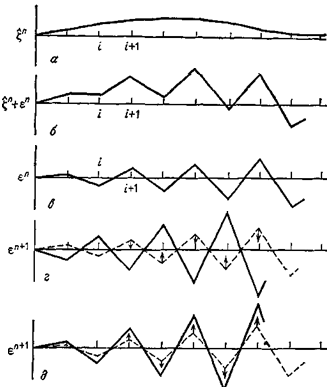
\includegraphics{{img/05/3.6}.png}
    \caption{Зростання похибки при використанні \eqref{eq:5.48}. а --- стаціонарний розв'язок на $n$-му шарі за часом; б --- збурений розв'язок на $n$-му шарі; в --- збурення на $n$-му шарі; г --- коливальне зростання похибки, пов'язане з надмірно великим кроком $\Delta t$ (динамічна нестійкість); д --- монотонне зростання похибки, обумовлене застосуванням центральних різниць для конвективного члена (статична нестійкість)}
    \label{fig:3.6}
\end{figure}

Після цього рівняння \eqref{eq:5.48} запишеться так:
\begin{equation}
    \label{eq:5.50}
    \frac{\zeta_i^{n + 1} - \zeta_i^n}{\Delta t} = - \frac{u \hat{\zeta}_{i + 1}^n - u \hat{\zeta}_{i - 1}^n}{2 \Delta x} + \alpha \frac{\hat{\zeta}_{i + 1}^n - 2 \hat{\zeta}_i^n + \hat{\zeta}_{i - 1}^n}{\Delta x^2} - \frac{u \epsilon_{i + 1}^n - u \epsilon_{i - 1}^n}{2 \Delta x} + \alpha \frac{\epsilon_{i + 1}^n - 2 \epsilon_i^n + \epsilon_{i - 1}^n}{\Delta x^2}.
\end{equation}

Сума перших двох членів у правій частині рівняння \eqref{eq:5.50} являє собою скінченно-різницеве значення $(\partial \hat{\zeta} / \partial t)_i^n$, рівне нулю в силу припущення, що на $n$-му часовому шарі існує стаціонарний розв'язок. Тоді рівняння \eqref{eq:5.50} зводиться до наступного:
\begin{equation}
    \label{eq:5.51}
    \zeta_i^{n + 1} - \zeta_i^n \equiv \Delta \zeta_i = \Delta t \frac{u \epsilon_{i + 1}^n - u \epsilon_{i - 1}^n}{2 \Delta x} + \alpha \Delta t \frac{\epsilon_{i + 1}^n - 2 \epsilon_i^n + \epsilon_{i - 1}^n}{\Delta x^2}.
\end{equation}

Перший член у правій частині рівняння \eqref{eq:5.51} дає зміну $\zeta$, обумовлену конвекцією, а другий --- обумовлену дифузією.
Розглянемо рівняння \eqref{eq:5.51} тільки з одним дифузійним членом і оцінимо його в точці $i$. Оскільки $\epsilon_{i + 1} > 0$, $\epsilon_i < 0$ і $\epsilon_{i - 1} > 0$, маємо
\begin{equation}
    \label{eq:5.52}
    \Delta \zeta_i = \alpha \Delta t \frac{\epsilon_{i + 1}^n - 2 \epsilon_i^n + \epsilon_{i - 1}^n}{\Delta x^2} > 0.
\end{equation}

Виходить, для всіх $\Delta t > 0$ приріст $\Delta \zeta_i$ додатній й прагне компенсувати від'ємне збурення $\epsilon_i$.
Аналогічно, розглядаючи $\Delta \zeta$ в точці $i + 1$, маємо $\epsilon_{i + 2} < 0$, $\epsilon_i < 0$ і $\epsilon_{i + 1} > 0$, тому
\begin{equation}
    \label{eq:5.53}
    \Delta \zeta_{i + 1} = \alpha \Delta t \frac{\epsilon_{i + 2}^n - 2 \epsilon_{i + 1}^n + \epsilon_i^n}{\Delta x^2} < 0.
\end{equation}
тобто додатнє збурення $\epsilon_{i + 1}$ коректується від'ємним приростом $\Delta \zeta_{i + 1}$. \medskip

Помітимо, що приріст $\Delta \zeta_i = \zeta_i^{n + 1} - \zeta_i^n$ (а також $\Delta \zeta_{i + 1}$ і т.д.) пропорційний кроку $\Delta t$. Якщо крок $\Delta t$ занадто великий, то поправка за рахунок збільшення $\Delta \zeta_i$  виявиться надмірною. Для таких занадто великих $\Delta t$ величина нового $\zeta_i^{n + 1}$ буде більше початкового збурення, як це показане на мал.~\ref{fig:3.6}(г):
\begin{equation}
    \label{eq:5.54}
    |\zeta_i^{n + 1}| > |\epsilon_i|
\end{equation}
і аналогічно
\begin{equation}
    \label{eq:5.55}
    |\zeta_{i \pm 1}^{n + 1}| > |\epsilon_{i \pm 1}|.
\end{equation}

Поява таких осциляцій наростаючої амплітуди, обумовлених надмірно великим кроком за часом, називається динамічною нестійкістю, яку можна усунути зменшенням кроку за часом, зробивши його менше деякого ``критичного кроку за часом'' $\Delta t_{\text{кр}}$. \medskip

Розглянемо тепер рівняння \eqref{eq:5.51} тільки з одним конвективним членом. Оцінимо це рівняння в точці $i$, вважаючи $u > 0$. Припустимо, що збурення коливається по $i$, а його амплітуда зростає з ростом $i$. Тому $u \epsilon_{i + 1} > 0$, $u \epsilon_{i - 1} > 0$, $u \epsilon_i < 0$ і 
\begin{equation}
    \label{eq:5.56}
    \Delta \zeta_i = - \Delta t \frac{u \epsilon_{i + 1}^n - u \epsilon_i^n}{2 \Delta x} < 0,
\end{equation}
тобто приріст $\zeta_i$, обумовлений конвекцією, від'ємний навіть при $\epsilon_i < 0$. Це означає, що похибка зростає монотонно (див. мал.~\ref{fig:3.6}(д)). Поява такої наростаючої похибки називається статичною нестійкістю, яку не можна усунути зменшенням кроку за часом і можна усунути тільки переходом до якої-небудь іншої скінченно-різницевої схеми. \medskip

Якщо просторовий напрямок зростання $\epsilon$ по відношенню до $u$ відрізняється від показаного на мал.~\ref{fig:3.6}, тобто якщо або $u < 0$, або амплітуда $\epsilon$ зменшується за $i$, то конвективний член стає статично стійким, але при достатньо великих $\Delta t$ ще може мати місце динамічна нестійкість. У будь-якій реальній задачі початкові похибки розподілені більш-менш випадково, і можна бути впевненим, що в деякий момент часу й у деякій точці їх розподіл буде схожий на зображений на мал.~\ref{fig:3.6} ``катастрофічний'' розподіл. \medskip

Якщо в рівняння \eqref{eq:5.51} входять і конвективний, і дифузійний члени, то вони взаємодіють. Як ми далі побачимо, для розглянутої різницевої схеми виникає обмеження на $\Delta t$, обумовлене дифузійним членом, і інше обмеження на $\Delta t$, що залежить від порівняльної величини статично нестійкого конвективного члена й статично стійкого дифузійного члена, тобто від числа Рейнольдса. 

\subsection{Дослідження стійкості}

Після того як був даний загальний опис стійкості, розглянемо методи дослідження стійкості, їх взаємозв'язки й їх порівняня. Ці методи будуть продемонстровані на прикладі різницевої схеми з різницями вперед за часом і центральними різницями по просторовій змінній у застосуванні до лінійного модельного рівняння \eqref{eq:2.18}.

\subsubsection{Метод дискретних збурень}

Метод дослідження стійкості, який ми називаємо методом дискретних збурень, являє собою узагальнення методу, уперше використаного Томом і Апельтом [1961] і розвиненого Томаном і Шевчиком [1966]. Цей метод повністю відповідає вже даному нами опису нестійкості. Він прямий і простий по ідеї, і може застосовуватися для аналізу як стійкості, так і властивості транспортивності, яке буде визначено далі. Ідея: у рівняння в деякій точці вводиться дискретне збурення величини $\zeta$ й прослідковується вплив цього збурення; скінченно-різницева схема буде стійкою, якщо збурення загасають. \medskip

Для простоти спочатку розглянемо рівняння \eqref{eq:2.18} тільки з дифузійним членом і припустимо, що знайдений стаціонарний розв'язок $\zeta_i^n = 0$ для всіх $i$. Введемо в розв'язок збурення $\epsilon$ й з \eqref{eq:2.18} за схемою з різницями вперед за часом і центральними різницями по просторовій змінній одержимо
\begin{equation}
    \label{eq:5.57}
    \frac{\zeta_i^{n + 1} - (\zeta_i^n + \epsilon)}{\Delta t} = \alpha \frac{\zeta_{i + 1}^n - 2(\zeta_i^n + \epsilon) + \zeta_{i - 1}^n}{\Delta x^2},
\end{equation}
або
\begin{equation}
    \label{eq:5.58}
    \frac{\zeta_i^{n + 1} - \epsilon}{\Delta t} = - \frac{2 \alpha \epsilon}{\Delta x^2},
\end{equation}
\begin{equation}
    \label{eq:5.59}
    \zeta_i^{n + 1} = \epsilon (1 - 2 d),
\end{equation}
де дифузійне число $d$ визначається рівністю
\begin{equation}
    \label{eq:5.60}
    d = \frac{\alpha \Delta t}{\Delta x^2}.
\end{equation}

В силу вимоги стійкості ці збурення повинні загасати. Для першого кроку за часом це приводить до умови
\begin{equation}
    \label{eq:5.61}
    |\zeta_i^{n + 1} / \epsilon | \le 1,
\end{equation}
або
\begin{equation}
    \label{eq:5.62}
    -1 \le 1 - 2 d \le 1.
\end{equation}

Права нерівність є результатом вимоги статичної стійкості й автоматично виконується при додатних $d$, тобто при $\alpha > 0$ й $\Delta t > 0$. Ліва нерівність є вимогою динамічної стійкості й виконується при $d \le 1$. Якщо, слідуючи Томану й Шевчику [1966], вимагати, щоб чисельний розв'язок моделював фізичне явище, не допускаючи осциляцій, обумовлених надмірно великим кроком за часом, тобто щоб
\begin{equation}
    \label{eq:5.63}
    \zeta_i^{n + 1} / \epsilon \ge 0 ,
\end{equation}
то випливає обмеження
\begin{equation}
    \label{eq:5.64}
    d \le 1/2.
\end{equation}

Нерівність \eqref{eq:5.63}, однак, не є умовою стійкості в розумінні зменшення амплітуди збурення. Якщо розглядати досить велику кількість шарів за часом, то буде потрібно виконання нерівності \eqref{eq:5.64}. Спочатку за схемою з різницями вперед за часом і центральними різницями по просторовій змінній (рівняння \eqref{eq:2.18}) обчислимо збурення в сусідніх точках:
\begin{equation}
    \label{eq:5.65}
    \zeta_{i \pm 1}^{n + 1} = d \epsilon.
\end{equation}

Для наступного шару за часом одержимо
\begin{equation}
    \label{eq:5.66}
    \zeta_i^{n + 2} = \zeta_i^{n + 1} + d ( \zeta_{i + 1}^{n + 1} - 2 \zeta_i^{n + 1} + \zeta_{i - 1}^{n + 1}) = \epsilon (1 - 2 d) + d (d \epsilon - 2 \epsilon(1 - 2d) + d \epsilon) = \epsilon (1 - 4 d + 6 d^2).
\end{equation}

Знову будемо вимагати, щоб мало місце нерівність
\begin{equation}
    \label{eq:5.67}
    |\zeta_i^{n + 2} / \epsilon | \le 1,
\end{equation}
звідки випливає
\begin{equation}
    \label{eq:5.68}
    -1 \le 1 - 4 d + 6 d^2 \le 1.
\end{equation}

Ліва нерівність виконується завжди, у той час як права накладає обмеження $d \le 2 / 3$. \medskip

Таким чином, розгляд першого часового шару приводить до умови $d \le 1$, а другого --- до умови $d \le 2 / 3$. Можна розглядати й наступні часові шари, які приводять до ще більш жорстких умов для $d$. Початкове одиничне збурення $\epsilon$ в точці $i$ асимптотично прямує до осцилюючого розподілу $\zeta_i = \pm \epsilon'$, де $\epsilon'$ --- деяке збурення меншої амплітуди, як показано на мал.~\ref{fig:3.7}.

\begin{figure}[H]
    \centering
    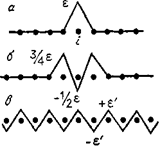
\includegraphics{{img/05/3.7}.png}
    \caption{Асимптотичне поширення одиничного збурення в у точці $i$ для рівняння дифузії, що розв'язується за схемою з різницями вперед за часом і із центральними різницями по просторовим змінним, а --- початкове збурення; б --- збурення після одного кроку за часом, $d = 3 / 4$; в --- збурення після дуже великої кількості кроків за часом.}
    \label{fig:3.7}
\end{figure}

Таким чином, видно, що найбільш жорстка умова для $d$ з'являється при такому типі розподілу збурень; починаючи розрахунки з таким осцилюючим збуренням $\epsilon'$, накладеним на $\zeta = 0$, і застосовуючи схему \eqref{eq:2.18} з різницями вперед за часом і центральними різницями по просторовій змінної, одержуємо
\begin{equation}
    \label{eq:5.69}
    \zeta_i^{n + 1} = \epsilon' + d(-\epsilon' - 2 \epsilon' - \epsilon') = \epsilon'(1 - 4 d).
\end{equation}

Вимога стійкості
\begin{equation}
    \label{eq:5.70}
    |\zeta_i^{n + 1} / \epsilon' | \le 1,
\end{equation}
дає
\begin{equation}
    \label{eq:5.71}
    -1 \le 1 - 4 d \le 1,
\end{equation}
або
\begin{equation}
    \label{eq:5.72}
    d \le 1 / 2.
\end{equation}

Для наступних часових шарів умова \eqref{eq:5.72} не міняється. Таким чином, це умова для великих значень часу еквівалентно умові \eqref{eq:5.64} --- умові відсутності осциляцій, обумовлених надмірно великим кроком за часом, у випадку ізольованого збурення. \medskip

З формули \eqref{eq:5.60} випливає, що при фіксованому кроці просторової сітки й фіксованому $\alpha$ умову $d \le 1 / 2$ накладає обмеження на крок за часом:
\begin{equation}
    \label{eq:5.73}
    \Delta t \le \frac{1}{2} \frac{\Delta x^2}{\alpha}    
\end{equation}

Відзначимо, що обмеження, що накладається умовою \eqref{eq:5.73}, є важким у розумінні витрат часу для чисельного розв'язку рівняння дифузії. Припустимо, що розрахунки ведуться з деяким просторовим кроком $\Delta x_1$ до деякого безрозмірного часу $T = N_1 \Delta t_1$, де $\Delta t_1 = \Delta x^2 / (2 \alpha)$ --- максимально можливий крок за часом. Якщо треба повторити розрахунки із удвічі меншим просторовим кроком $\Delta x_2 / \Delta x_1 / 2$ (наприклад, для того, щоб проконтролювати зменшення похибок апроксимації), то треба брати крок за часом $\Delta t_2 = \Delta t_1 / 4$. Виходить, щоб досягти того ж значення безрозмірного часу $T$, буде потрібно вчетверо більше кроків за часом. Крім того, для розрахунків кожного часового шару буде потрібно вдвічі більше часу, тому що $\Delta x_2 = \Delta x_1 / 2$, а це означає, що число розрахункових точок у досліджуваній області зросло вдвічі. Таким чином, для одномірного випадку зменшення вдвічі кроку просторової сітки збільшує витрати машинного часу у 8 разів! \medskip

У двовимірній задачі зменшення вдвічі кроків $\Delta x$ і $\Delta y$ збільшує число розрахункових точок у чотири рази, збільшуючи тим самим необхідний машинний час в 16 раз. У тривимірній задачі дифузії зменшення всіх трьох просторових кроків удвічі збільшує машинний час в 32 рази. У загальному випадку зменшення розміру кроку з $\Delta x_1$ до $\Delta x_2$ при розв'язку $D$-мірної задачі дифузії з використанням явної схеми з різницями вперед за часом і центральними різницями по просторових змінних збільшує машинний час у $(\Delta x_1 / \Delta x_2)^{2 + D}$ разів. Ясно, що методи, у яких вдається уникнути умови стійкості \eqref{eq:5.73}, були б досить бажані. \medskip

В наведених вище міркуваннях припущення про стаціонарність розв'язку несуттєве. Якщо зі збуреного рівняння відняти повне незбурене нестаціонарне рівняння, то вийде рівняння для зміни похибки
\begin{equation}
    \epsilon_i^{n + 1} = d (\epsilon_{i + 1}^n - 2 \epsilon_i^n + \epsilon_{i - 1}^n) + \epsilon_i^n
\end{equation}
з умовою стійкості $|\epsilon_i^{n + 1} / \epsilon_i^n| \le 1$ і т.д. Результати в цьому випадку будуть ті ж, що й вище. \medskip

Розглянемо тепер рівняння \eqref{eq:2.18} з конвективним й дифузійним членами й без обмеження загальності покладемо $u > 0$ (Якщо $u < 0$, то зміниться роль індексів $i + 1$ і $i - 1$). Знову застосуємо схему з різницями вперед за часом і центральними різницями по просторовій змінній, накладаючи на $\zeta_i^{n + 1}$ в точці $i$ збурення $\epsilon$, що дасть
\begin{equation}
    \label{eq:5.75}
    \frac{\zeta_i^{n + 1} - (\zeta_i^n + \epsilon)}{\Delta t} = - \frac{u \zeta_{i + 1}^n - u \zeta_{i - 1}^n}{2 \Delta x} + \alpha \left( \frac{\zeta_{i + 1}^n - 2 (\zeta_i^n + \epsilon) + \zeta_{i - 1}^n}{\Delta x^2} \right)
\end{equation}

Дослідження цього рівняння не дає додаткової інформації в порівнянні з попереднім аналізом рівняння з одним тільки дифузійним членом, тому що на конвективних членах у точках $i \pm 1$ не позначається збурення в точці $i$. Застосовуючи схему з різницями вперед за часом і центральними різницями по просторовій змінній і в точці $i + 1$, одержуємо
\begin{equation}
    \label{eq:5.76}
    \zeta_{i + 1}^{n + 1} = - \frac{\Delta t}{2 \Delta x} ( u \zeta_{i + 2}^n - u(\zeta_i^n + \epsilon)) + \frac{\alpha \Delta t}{\Delta x^2} (\zeta_{i + 2}^n - 2 \zeta_{i + 1}^n + \zeta_i^n + \epsilon) + \zeta_{i + 1}^n.
\end{equation}
або
\begin{equation}
    \label{eq:5.77}
    \zeta_{i + 1}^{n + 1} = \frac{C \epsilon}{2} + d \epsilon
\end{equation}
де $C = u \Delta t / \Delta x$ --- число Куранта, a $d = \alpha \Delta t / \Delta x^2$, як і раніше. Для стійкості знову будемо вимагати, щоб
\begin{equation}
    \label{eq:5.78}
    |\zeta_{i + 1}^{n + 1} / \epsilon| \le 1,
\end{equation}
або
\begin{equation}
    \label{eq:5.79}
    -1 \le \frac{C}{2} + d \le 1.
\end{equation}

Ліва нерівність автоматично виконується при $u > 0$. Права нерівність (вимога статичної стійкості) дає іншу необхідну умову стійкості:
\begin{equation}
    u \Delta t / \Delta x + 2 \alpha \Delta t / \Delta x^2 \le 2,
\end{equation}
або
\begin{equation}
    \label{eq:5.80}
    \Delta t \le \frac{2}{2 \alpha / \Delta x^2 + u / \Delta x}.    
\end{equation}

Звернувшись тепер до точки $i - 1$, одержимо
\begin{equation}
    \label{eq:5.81}
    \zeta_{i - 1}^{n + 1} = - \frac{C \epsilon}{2} + d \epsilon
\end{equation}
і вимога стійкості $|\zeta_{i - 1}^{n + 1} / \epsilon| \le 1$ тут дає
\begin{equation}
    \label{eq:5.82}
    -1 \le - \frac{C}{2} + d \le 1.
\end{equation}

Розглядаючи спочатку праву нерівність \eqref{eq:5.82} (статична стійкість), одержуємо
\begin{equation}
    \label{eq:5.83}
    \Delta t \left( \frac{2 \alpha}{\Delta x^2} - \frac{u}{\Delta x} \right) \le 2.    
\end{equation}

Якщо член у дужках від'ємний, то ця нерівність буде справедливо для всіх $\Delta t > 0$ , якщо ж цей член додатній, то одержуємо
\begin{equation}
    \label{eq:5.84}
    \Delta t \le \frac{2}{2 \alpha / \Delta x^2 - u / \Delta x}.    
\end{equation}

Оскільки знаменник додатній, умова \eqref{eq:5.84} менш жорстка, ніж \eqref{eq:5.80}, і тому перекривається нею. \medskip

Дослідження лівої нерівності \eqref{eq:5.82} (динамічна стійкість) дає
\begin{equation}
    \label{eq:5.85}
    -2 \le \Delta t \left( \frac{2 \alpha}{\Delta x^2} - \frac{u}{\Delta x} \right)
\end{equation}
Якщо член у дужках додатній, то ця нерівність виконується для всіх $\Delta t > 0$ , якщо ж цей член від'ємний, то одержуємо
\begin{equation}
    \label{eq:5.86}
    \Delta t \le \frac{2}{u / \Delta x - 2 \alpha / \Delta x^2}.
\end{equation}
де знаменник додатній. Умова \eqref{eq:5.86} також менш жорстка, ніж \eqref{eq:5.80}, і тому перекривається нею. \medskip

Таким чином, з аналізу стійкості рівняння, що включає конвективний і дифузійний члени, за допомогою методу дискретних збурень випливають дві необхідні умови --- рівняння \eqref{eq:5.73} і \eqref{eq:5.80}. Якщо поширити цей аналіз на наступні шари за часом, то можуть з'явитися інші більш обмежувальні умови, але метод аналізу при цьому стає дуже незручним. Помітимо (і це буде показано нижче), що аналіз стійкості по фон Нейману дає іншу умова (нерівність $C^2 \le 2 d$). \medskip

Крім того, якщо додержуватися роботи Томана й Шевчика [1966] і додатково вимагати відсутності в точці $i - 1$ осциляцій, обумовлених надмірно великим  кроком за часом, то повинне бути
\begin{equation}
    \label{eq:5.87}
    \zeta_{i - 1}^{n + 1} / \epsilon > 0,
\end{equation}
а рівняння \eqref{eq:5.81} дасть
\begin{equation}
    \label{eq:5.88}
    - C / 2 + d \ge 0,
\end{equation}
тобто
\begin{equation}
    \label{eq:5.89}
    - u \Delta t / \Delta x + 2 \alpha \Delta t / \Delta x^2 \ge 0,
\end{equation}
або
\begin{equation}
    \label{eq:5.90}
    u \Delta t / \alpha \le 2.
\end{equation}

У рівнянні переносу вихору $\alpha = 1 / \text{Re}$ й член $u \Delta x / \alpha$ являє собою сіткове число Рейнольдса $\text{Re}_c$. Таким чином, $\text{Re}_c$ є число Рейнольдса, отримане по локальній швидкості й характерній довжині, рівній розміру кроку просторової сітки $\Delta x$. Для відсутності осциляцій, обумовлених надмірно великим кроком за часом, потрібно, щоб
\begin{equation}
    \label{eq:5.91}
    \text{Re}_c \le 2
\end{equation}
незалежно від $\Delta t$. Якщо вимогу відсутності осциляцій \eqref{eq:5.90} скомбінувати з умовою \eqref{eq:5.73}, що накладається дифузією, то в результаті виходять наступні обмеження: число Куранта $C = u \delta t / \Delta x \le 1$ й $\Delta t \le 2 \alpha / u^2$. Як побачимо надалі, ці обмеження є правильними.

\subsection{Завдання для самостійної роботи}

\shortHomeworkDescription{Використовуючи метод дискретних збурень, дослідити стійкість схеми з різницями проти потоку
\begin{equation}
    \label{eq:5.92}
    \frac{\zeta_i^{n + 1} - \zeta_i^n}{\Delta t} = - \frac{u \zeta_i^n - u \zeta_{i - 1}^n}{\Delta z}, \quad u > 0
\end{equation}
що відповідає модельному рівнянню руху нев'язкої рідини. Показати, що умова стійкості накладає на число Куранта обмеження $C = u \Delta t / \Delta x \le 1$ й що вона включає критерій відсутності осциляцій, обумовлених надмірно великим кроком за часом.}


%% last slide
\begin{frame}{$\left.\right.$}
  \centering \Huge
  \emph{Дякуємо за увагу!}
\end{frame}
%% last slide

\end{document}

\usepackage[explicit]{hulianytskyi}
\begin{document}
\title{Узагальнене оптимальне керування}
\author{Гуляницький А.~Л.\footnote{Гуляницький Андрій Леонідович, \texttt{andriy.hul@gmail.com}}}
\date{15 жовтня -- 5 листопада 2019 р.}
\maketitle
\tableofcontents
\thispagestyle{empty}
\setcounter{section}{1}
% \setcounter{subsection}{0}
\section{Поняття стійкості різницевих схем}

\shortLectureDescription{Поняття стійкості різницевих схем. Причини і види розповсюдження збурення. Поняття асимптотичної збіжності різницевих схем. Метод дискретних збурень. \cite{rouch1980, sam1983, richtmyer1972, kollatz}}

\subsection{Опис нестійкості}

Для ознайомлення з деякими феноменологічними аспектами чисельної нестійкості розглянемо одномірне модельне лінійне рівняння для $\zeta$. На мал.~\ref{fig:3.6}(а) показаний стаціонарний розв'язок $\hat{\zeta}^n$  на $n$-му часовому шарі, а на мал.~\ref{fig:3.6}(б) --- накладення на $\zeta^n$ збурення $\epsilon$, форма якого представлена на мал.~\ref{fig:3.6}(в). Такі збурення можуть породжуватися або машинними похибками округлення, або поперечними рухами у реальній двовимірній задачі. Використовуючи схему з різницями вперед за часом і центральними різницями по просторовій змінної, простежимо за розвитком накладеного збурення. Лінійне модельне рівняння в консервативній формі має вигляд
\begin{equation*}
    \frac{\partial \zeta}{\partial t} = - \frac{\partial (u \zeta)}{\partial x} + \alpha \frac{\partial^2 \zeta}{\partial x^2}
\end{equation*}
а різницеве --- вигляд
\begin{equation}
    \label{eq:5.48}
    \frac{\zeta_i^{n + 1} - \zeta_i^n}{\Delta t} = - \frac{u \zeta_{i + 1}^n - u \zeta_{i - 1}^n}{2 \Delta x} + \alpha \frac{\zeta_{i + 1}^n - 2 \zeta_i^n + \zeta_{i - 1}^n}{\Delta x^2}
\end{equation}
Представимо величину $\zeta$ як суму стаціонарної компоненти $\hat{\zeta}$ й збурення $\epsilon$:
\begin{equation}
    \label{eq:5.49}
    \zeta_i^n = \hat{\zeta}_i^n + \epsilon_i.
\end{equation}
 
\begin{figure}[H]
    \centering
    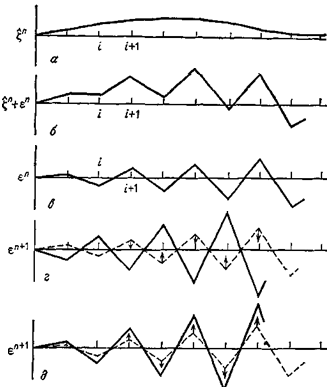
\includegraphics{{img/05/3.6}.png}
    \caption{Зростання похибки при використанні \eqref{eq:5.48}. а --- стаціонарний розв'язок на $n$-му шарі за часом; б --- збурений розв'язок на $n$-му шарі; в --- збурення на $n$-му шарі; г --- коливальне зростання похибки, пов'язане з надмірно великим кроком $\Delta t$ (динамічна нестійкість); д --- монотонне зростання похибки, обумовлене застосуванням центральних різниць для конвективного члена (статична нестійкість)}
    \label{fig:3.6}
\end{figure}

Після цього рівняння \eqref{eq:5.48} запишеться так:
\begin{equation}
    \label{eq:5.50}
    \frac{\zeta_i^{n + 1} - \zeta_i^n}{\Delta t} = - \frac{u \hat{\zeta}_{i + 1}^n - u \hat{\zeta}_{i - 1}^n}{2 \Delta x} + \alpha \frac{\hat{\zeta}_{i + 1}^n - 2 \hat{\zeta}_i^n + \hat{\zeta}_{i - 1}^n}{\Delta x^2} - \frac{u \epsilon_{i + 1}^n - u \epsilon_{i - 1}^n}{2 \Delta x} + \alpha \frac{\epsilon_{i + 1}^n - 2 \epsilon_i^n + \epsilon_{i - 1}^n}{\Delta x^2}.
\end{equation}

Сума перших двох членів у правій частині рівняння \eqref{eq:5.50} являє собою скінченно-різницеве значення $(\partial \hat{\zeta} / \partial t)_i^n$, рівне нулю в силу припущення, що на $n$-му часовому шарі існує стаціонарний розв'язок. Тоді рівняння \eqref{eq:5.50} зводиться до наступного:
\begin{equation}
    \label{eq:5.51}
    \zeta_i^{n + 1} - \zeta_i^n \equiv \Delta \zeta_i = \Delta t \frac{u \epsilon_{i + 1}^n - u \epsilon_{i - 1}^n}{2 \Delta x} + \alpha \Delta t \frac{\epsilon_{i + 1}^n - 2 \epsilon_i^n + \epsilon_{i - 1}^n}{\Delta x^2}.
\end{equation}

Перший член у правій частині рівняння \eqref{eq:5.51} дає зміну $\zeta$, обумовлену конвекцією, а другий --- обумовлену дифузією.
Розглянемо рівняння \eqref{eq:5.51} тільки з одним дифузійним членом і оцінимо його в точці $i$. Оскільки $\epsilon_{i + 1} > 0$, $\epsilon_i < 0$ і $\epsilon_{i - 1} > 0$, маємо
\begin{equation}
    \label{eq:5.52}
    \Delta \zeta_i = \alpha \Delta t \frac{\epsilon_{i + 1}^n - 2 \epsilon_i^n + \epsilon_{i - 1}^n}{\Delta x^2} > 0.
\end{equation}

Виходить, для всіх $\Delta t > 0$ приріст $\Delta \zeta_i$ додатній й прагне компенсувати від'ємне збурення $\epsilon_i$.
Аналогічно, розглядаючи $\Delta \zeta$ в точці $i + 1$, маємо $\epsilon_{i + 2} < 0$, $\epsilon_i < 0$ і $\epsilon_{i + 1} > 0$, тому
\begin{equation}
    \label{eq:5.53}
    \Delta \zeta_{i + 1} = \alpha \Delta t \frac{\epsilon_{i + 2}^n - 2 \epsilon_{i + 1}^n + \epsilon_i^n}{\Delta x^2} < 0.
\end{equation}
тобто додатнє збурення $\epsilon_{i + 1}$ коректується від'ємним приростом $\Delta \zeta_{i + 1}$. \medskip

Помітимо, що приріст $\Delta \zeta_i = \zeta_i^{n + 1} - \zeta_i^n$ (а також $\Delta \zeta_{i + 1}$ і т.д.) пропорційний кроку $\Delta t$. Якщо крок $\Delta t$ занадто великий, то поправка за рахунок збільшення $\Delta \zeta_i$  виявиться надмірною. Для таких занадто великих $\Delta t$ величина нового $\zeta_i^{n + 1}$ буде більше початкового збурення, як це показане на мал.~\ref{fig:3.6}(г):
\begin{equation}
    \label{eq:5.54}
    |\zeta_i^{n + 1}| > |\epsilon_i|
\end{equation}
і аналогічно
\begin{equation}
    \label{eq:5.55}
    |\zeta_{i \pm 1}^{n + 1}| > |\epsilon_{i \pm 1}|.
\end{equation}

Поява таких осциляцій наростаючої амплітуди, обумовлених надмірно великим кроком за часом, називається динамічною нестійкістю, яку можна усунути зменшенням кроку за часом, зробивши його менше деякого ``критичного кроку за часом'' $\Delta t_{\text{кр}}$. \medskip

Розглянемо тепер рівняння \eqref{eq:5.51} тільки з одним конвективним членом. Оцінимо це рівняння в точці $i$, вважаючи $u > 0$. Припустимо, що збурення коливається по $i$, а його амплітуда зростає з ростом $i$. Тому $u \epsilon_{i + 1} > 0$, $u \epsilon_{i - 1} > 0$, $u \epsilon_i < 0$ і 
\begin{equation}
    \label{eq:5.56}
    \Delta \zeta_i = - \Delta t \frac{u \epsilon_{i + 1}^n - u \epsilon_i^n}{2 \Delta x} < 0,
\end{equation}
тобто приріст $\zeta_i$, обумовлений конвекцією, від'ємний навіть при $\epsilon_i < 0$. Це означає, що похибка зростає монотонно (див. мал.~\ref{fig:3.6}(д)). Поява такої наростаючої похибки називається статичною нестійкістю, яку не можна усунути зменшенням кроку за часом і можна усунути тільки переходом до якої-небудь іншої скінченно-різницевої схеми. \medskip

Якщо просторовий напрямок зростання $\epsilon$ по відношенню до $u$ відрізняється від показаного на мал.~\ref{fig:3.6}, тобто якщо або $u < 0$, або амплітуда $\epsilon$ зменшується за $i$, то конвективний член стає статично стійким, але при достатньо великих $\Delta t$ ще може мати місце динамічна нестійкість. У будь-якій реальній задачі початкові похибки розподілені більш-менш випадково, і можна бути впевненим, що в деякий момент часу й у деякій точці їх розподіл буде схожий на зображений на мал.~\ref{fig:3.6} ``катастрофічний'' розподіл. \medskip

Якщо в рівняння \eqref{eq:5.51} входять і конвективний, і дифузійний члени, то вони взаємодіють. Як ми далі побачимо, для розглянутої різницевої схеми виникає обмеження на $\Delta t$, обумовлене дифузійним членом, і інше обмеження на $\Delta t$, що залежить від порівняльної величини статично нестійкого конвективного члена й статично стійкого дифузійного члена, тобто від числа Рейнольдса. 

\subsection{Дослідження стійкості}

Після того як був даний загальний опис стійкості, розглянемо методи дослідження стійкості, їх взаємозв'язки й їх порівняня. Ці методи будуть продемонстровані на прикладі різницевої схеми з різницями вперед за часом і центральними різницями по просторовій змінній у застосуванні до лінійного модельного рівняння \eqref{eq:2.18}.

\subsubsection{Метод дискретних збурень}

Метод дослідження стійкості, який ми називаємо методом дискретних збурень, являє собою узагальнення методу, уперше використаного Томом і Апельтом [1961] і розвиненого Томаном і Шевчиком [1966]. Цей метод повністю відповідає вже даному нами опису нестійкості. Він прямий і простий по ідеї, і може застосовуватися для аналізу як стійкості, так і властивості транспортивності, яке буде визначено далі. Ідея: у рівняння в деякій точці вводиться дискретне збурення величини $\zeta$ й прослідковується вплив цього збурення; скінченно-різницева схема буде стійкою, якщо збурення загасають. \medskip

Для простоти спочатку розглянемо рівняння \eqref{eq:2.18} тільки з дифузійним членом і припустимо, що знайдений стаціонарний розв'язок $\zeta_i^n = 0$ для всіх $i$. Введемо в розв'язок збурення $\epsilon$ й з \eqref{eq:2.18} за схемою з різницями вперед за часом і центральними різницями по просторовій змінній одержимо
\begin{equation}
    \label{eq:5.57}
    \frac{\zeta_i^{n + 1} - (\zeta_i^n + \epsilon)}{\Delta t} = \alpha \frac{\zeta_{i + 1}^n - 2(\zeta_i^n + \epsilon) + \zeta_{i - 1}^n}{\Delta x^2},
\end{equation}
або
\begin{equation}
    \label{eq:5.58}
    \frac{\zeta_i^{n + 1} - \epsilon}{\Delta t} = - \frac{2 \alpha \epsilon}{\Delta x^2},
\end{equation}
\begin{equation}
    \label{eq:5.59}
    \zeta_i^{n + 1} = \epsilon (1 - 2 d),
\end{equation}
де дифузійне число $d$ визначається рівністю
\begin{equation}
    \label{eq:5.60}
    d = \frac{\alpha \Delta t}{\Delta x^2}.
\end{equation}

В силу вимоги стійкості ці збурення повинні загасати. Для першого кроку за часом це приводить до умови
\begin{equation}
    \label{eq:5.61}
    |\zeta_i^{n + 1} / \epsilon | \le 1,
\end{equation}
або
\begin{equation}
    \label{eq:5.62}
    -1 \le 1 - 2 d \le 1.
\end{equation}

Права нерівність є результатом вимоги статичної стійкості й автоматично виконується при додатних $d$, тобто при $\alpha > 0$ й $\Delta t > 0$. Ліва нерівність є вимогою динамічної стійкості й виконується при $d \le 1$. Якщо, слідуючи Томану й Шевчику [1966], вимагати, щоб чисельний розв'язок моделював фізичне явище, не допускаючи осциляцій, обумовлених надмірно великим кроком за часом, тобто щоб
\begin{equation}
    \label{eq:5.63}
    \zeta_i^{n + 1} / \epsilon \ge 0 ,
\end{equation}
то випливає обмеження
\begin{equation}
    \label{eq:5.64}
    d \le 1/2.
\end{equation}

Нерівність \eqref{eq:5.63}, однак, не є умовою стійкості в розумінні зменшення амплітуди збурення. Якщо розглядати досить велику кількість шарів за часом, то буде потрібно виконання нерівності \eqref{eq:5.64}. Спочатку за схемою з різницями вперед за часом і центральними різницями по просторовій змінній (рівняння \eqref{eq:2.18}) обчислимо збурення в сусідніх точках:
\begin{equation}
    \label{eq:5.65}
    \zeta_{i \pm 1}^{n + 1} = d \epsilon.
\end{equation}

Для наступного шару за часом одержимо
\begin{equation}
    \label{eq:5.66}
    \zeta_i^{n + 2} = \zeta_i^{n + 1} + d ( \zeta_{i + 1}^{n + 1} - 2 \zeta_i^{n + 1} + \zeta_{i - 1}^{n + 1}) = \epsilon (1 - 2 d) + d (d \epsilon - 2 \epsilon(1 - 2d) + d \epsilon) = \epsilon (1 - 4 d + 6 d^2).
\end{equation}

Знову будемо вимагати, щоб мало місце нерівність
\begin{equation}
    \label{eq:5.67}
    |\zeta_i^{n + 2} / \epsilon | \le 1,
\end{equation}
звідки випливає
\begin{equation}
    \label{eq:5.68}
    -1 \le 1 - 4 d + 6 d^2 \le 1.
\end{equation}

Ліва нерівність виконується завжди, у той час як права накладає обмеження $d \le 2 / 3$. \medskip

Таким чином, розгляд першого часового шару приводить до умови $d \le 1$, а другого --- до умови $d \le 2 / 3$. Можна розглядати й наступні часові шари, які приводять до ще більш жорстких умов для $d$. Початкове одиничне збурення $\epsilon$ в точці $i$ асимптотично прямує до осцилюючого розподілу $\zeta_i = \pm \epsilon'$, де $\epsilon'$ --- деяке збурення меншої амплітуди, як показано на мал.~\ref{fig:3.7}.

\begin{figure}[H]
    \centering
    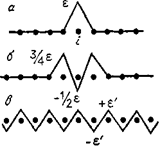
\includegraphics{{img/05/3.7}.png}
    \caption{Асимптотичне поширення одиничного збурення в у точці $i$ для рівняння дифузії, що розв'язується за схемою з різницями вперед за часом і із центральними різницями по просторовим змінним, а --- початкове збурення; б --- збурення після одного кроку за часом, $d = 3 / 4$; в --- збурення після дуже великої кількості кроків за часом.}
    \label{fig:3.7}
\end{figure}

Таким чином, видно, що найбільш жорстка умова для $d$ з'являється при такому типі розподілу збурень; починаючи розрахунки з таким осцилюючим збуренням $\epsilon'$, накладеним на $\zeta = 0$, і застосовуючи схему \eqref{eq:2.18} з різницями вперед за часом і центральними різницями по просторовій змінної, одержуємо
\begin{equation}
    \label{eq:5.69}
    \zeta_i^{n + 1} = \epsilon' + d(-\epsilon' - 2 \epsilon' - \epsilon') = \epsilon'(1 - 4 d).
\end{equation}

Вимога стійкості
\begin{equation}
    \label{eq:5.70}
    |\zeta_i^{n + 1} / \epsilon' | \le 1,
\end{equation}
дає
\begin{equation}
    \label{eq:5.71}
    -1 \le 1 - 4 d \le 1,
\end{equation}
або
\begin{equation}
    \label{eq:5.72}
    d \le 1 / 2.
\end{equation}

Для наступних часових шарів умова \eqref{eq:5.72} не міняється. Таким чином, це умова для великих значень часу еквівалентно умові \eqref{eq:5.64} --- умові відсутності осциляцій, обумовлених надмірно великим кроком за часом, у випадку ізольованого збурення. \medskip

З формули \eqref{eq:5.60} випливає, що при фіксованому кроці просторової сітки й фіксованому $\alpha$ умову $d \le 1 / 2$ накладає обмеження на крок за часом:
\begin{equation}
    \label{eq:5.73}
    \Delta t \le \frac{1}{2} \frac{\Delta x^2}{\alpha}    
\end{equation}

Відзначимо, що обмеження, що накладається умовою \eqref{eq:5.73}, є важким у розумінні витрат часу для чисельного розв'язку рівняння дифузії. Припустимо, що розрахунки ведуться з деяким просторовим кроком $\Delta x_1$ до деякого безрозмірного часу $T = N_1 \Delta t_1$, де $\Delta t_1 = \Delta x^2 / (2 \alpha)$ --- максимально можливий крок за часом. Якщо треба повторити розрахунки із удвічі меншим просторовим кроком $\Delta x_2 / \Delta x_1 / 2$ (наприклад, для того, щоб проконтролювати зменшення похибок апроксимації), то треба брати крок за часом $\Delta t_2 = \Delta t_1 / 4$. Виходить, щоб досягти того ж значення безрозмірного часу $T$, буде потрібно вчетверо більше кроків за часом. Крім того, для розрахунків кожного часового шару буде потрібно вдвічі більше часу, тому що $\Delta x_2 = \Delta x_1 / 2$, а це означає, що число розрахункових точок у досліджуваній області зросло вдвічі. Таким чином, для одномірного випадку зменшення вдвічі кроку просторової сітки збільшує витрати машинного часу у 8 разів! \medskip

У двовимірній задачі зменшення вдвічі кроків $\Delta x$ і $\Delta y$ збільшує число розрахункових точок у чотири рази, збільшуючи тим самим необхідний машинний час в 16 раз. У тривимірній задачі дифузії зменшення всіх трьох просторових кроків удвічі збільшує машинний час в 32 рази. У загальному випадку зменшення розміру кроку з $\Delta x_1$ до $\Delta x_2$ при розв'язку $D$-мірної задачі дифузії з використанням явної схеми з різницями вперед за часом і центральними різницями по просторових змінних збільшує машинний час у $(\Delta x_1 / \Delta x_2)^{2 + D}$ разів. Ясно, що методи, у яких вдається уникнути умови стійкості \eqref{eq:5.73}, були б досить бажані. \medskip

В наведених вище міркуваннях припущення про стаціонарність розв'язку несуттєве. Якщо зі збуреного рівняння відняти повне незбурене нестаціонарне рівняння, то вийде рівняння для зміни похибки
\begin{equation}
    \epsilon_i^{n + 1} = d (\epsilon_{i + 1}^n - 2 \epsilon_i^n + \epsilon_{i - 1}^n) + \epsilon_i^n
\end{equation}
з умовою стійкості $|\epsilon_i^{n + 1} / \epsilon_i^n| \le 1$ і т.д. Результати в цьому випадку будуть ті ж, що й вище. \medskip

Розглянемо тепер рівняння \eqref{eq:2.18} з конвективним й дифузійним членами й без обмеження загальності покладемо $u > 0$ (Якщо $u < 0$, то зміниться роль індексів $i + 1$ і $i - 1$). Знову застосуємо схему з різницями вперед за часом і центральними різницями по просторовій змінній, накладаючи на $\zeta_i^{n + 1}$ в точці $i$ збурення $\epsilon$, що дасть
\begin{equation}
    \label{eq:5.75}
    \frac{\zeta_i^{n + 1} - (\zeta_i^n + \epsilon)}{\Delta t} = - \frac{u \zeta_{i + 1}^n - u \zeta_{i - 1}^n}{2 \Delta x} + \alpha \left( \frac{\zeta_{i + 1}^n - 2 (\zeta_i^n + \epsilon) + \zeta_{i - 1}^n}{\Delta x^2} \right)
\end{equation}

Дослідження цього рівняння не дає додаткової інформації в порівнянні з попереднім аналізом рівняння з одним тільки дифузійним членом, тому що на конвективних членах у точках $i \pm 1$ не позначається збурення в точці $i$. Застосовуючи схему з різницями вперед за часом і центральними різницями по просторовій змінній і в точці $i + 1$, одержуємо
\begin{equation}
    \label{eq:5.76}
    \zeta_{i + 1}^{n + 1} = - \frac{\Delta t}{2 \Delta x} ( u \zeta_{i + 2}^n - u(\zeta_i^n + \epsilon)) + \frac{\alpha \Delta t}{\Delta x^2} (\zeta_{i + 2}^n - 2 \zeta_{i + 1}^n + \zeta_i^n + \epsilon) + \zeta_{i + 1}^n.
\end{equation}
або
\begin{equation}
    \label{eq:5.77}
    \zeta_{i + 1}^{n + 1} = \frac{C \epsilon}{2} + d \epsilon
\end{equation}
де $C = u \Delta t / \Delta x$ --- число Куранта, a $d = \alpha \Delta t / \Delta x^2$, як і раніше. Для стійкості знову будемо вимагати, щоб
\begin{equation}
    \label{eq:5.78}
    |\zeta_{i + 1}^{n + 1} / \epsilon| \le 1,
\end{equation}
або
\begin{equation}
    \label{eq:5.79}
    -1 \le \frac{C}{2} + d \le 1.
\end{equation}

Ліва нерівність автоматично виконується при $u > 0$. Права нерівність (вимога статичної стійкості) дає іншу необхідну умову стійкості:
\begin{equation}
    u \Delta t / \Delta x + 2 \alpha \Delta t / \Delta x^2 \le 2,
\end{equation}
або
\begin{equation}
    \label{eq:5.80}
    \Delta t \le \frac{2}{2 \alpha / \Delta x^2 + u / \Delta x}.    
\end{equation}

Звернувшись тепер до точки $i - 1$, одержимо
\begin{equation}
    \label{eq:5.81}
    \zeta_{i - 1}^{n + 1} = - \frac{C \epsilon}{2} + d \epsilon
\end{equation}
і вимога стійкості $|\zeta_{i - 1}^{n + 1} / \epsilon| \le 1$ тут дає
\begin{equation}
    \label{eq:5.82}
    -1 \le - \frac{C}{2} + d \le 1.
\end{equation}

Розглядаючи спочатку праву нерівність \eqref{eq:5.82} (статична стійкість), одержуємо
\begin{equation}
    \label{eq:5.83}
    \Delta t \left( \frac{2 \alpha}{\Delta x^2} - \frac{u}{\Delta x} \right) \le 2.    
\end{equation}

Якщо член у дужках від'ємний, то ця нерівність буде справедливо для всіх $\Delta t > 0$ , якщо ж цей член додатній, то одержуємо
\begin{equation}
    \label{eq:5.84}
    \Delta t \le \frac{2}{2 \alpha / \Delta x^2 - u / \Delta x}.    
\end{equation}

Оскільки знаменник додатній, умова \eqref{eq:5.84} менш жорстка, ніж \eqref{eq:5.80}, і тому перекривається нею. \medskip

Дослідження лівої нерівності \eqref{eq:5.82} (динамічна стійкість) дає
\begin{equation}
    \label{eq:5.85}
    -2 \le \Delta t \left( \frac{2 \alpha}{\Delta x^2} - \frac{u}{\Delta x} \right)
\end{equation}
Якщо член у дужках додатній, то ця нерівність виконується для всіх $\Delta t > 0$ , якщо ж цей член від'ємний, то одержуємо
\begin{equation}
    \label{eq:5.86}
    \Delta t \le \frac{2}{u / \Delta x - 2 \alpha / \Delta x^2}.
\end{equation}
де знаменник додатній. Умова \eqref{eq:5.86} також менш жорстка, ніж \eqref{eq:5.80}, і тому перекривається нею. \medskip

Таким чином, з аналізу стійкості рівняння, що включає конвективний і дифузійний члени, за допомогою методу дискретних збурень випливають дві необхідні умови --- рівняння \eqref{eq:5.73} і \eqref{eq:5.80}. Якщо поширити цей аналіз на наступні шари за часом, то можуть з'явитися інші більш обмежувальні умови, але метод аналізу при цьому стає дуже незручним. Помітимо (і це буде показано нижче), що аналіз стійкості по фон Нейману дає іншу умова (нерівність $C^2 \le 2 d$). \medskip

Крім того, якщо додержуватися роботи Томана й Шевчика [1966] і додатково вимагати відсутності в точці $i - 1$ осциляцій, обумовлених надмірно великим  кроком за часом, то повинне бути
\begin{equation}
    \label{eq:5.87}
    \zeta_{i - 1}^{n + 1} / \epsilon > 0,
\end{equation}
а рівняння \eqref{eq:5.81} дасть
\begin{equation}
    \label{eq:5.88}
    - C / 2 + d \ge 0,
\end{equation}
тобто
\begin{equation}
    \label{eq:5.89}
    - u \Delta t / \Delta x + 2 \alpha \Delta t / \Delta x^2 \ge 0,
\end{equation}
або
\begin{equation}
    \label{eq:5.90}
    u \Delta t / \alpha \le 2.
\end{equation}

У рівнянні переносу вихору $\alpha = 1 / \text{Re}$ й член $u \Delta x / \alpha$ являє собою сіткове число Рейнольдса $\text{Re}_c$. Таким чином, $\text{Re}_c$ є число Рейнольдса, отримане по локальній швидкості й характерній довжині, рівній розміру кроку просторової сітки $\Delta x$. Для відсутності осциляцій, обумовлених надмірно великим кроком за часом, потрібно, щоб
\begin{equation}
    \label{eq:5.91}
    \text{Re}_c \le 2
\end{equation}
незалежно від $\Delta t$. Якщо вимогу відсутності осциляцій \eqref{eq:5.90} скомбінувати з умовою \eqref{eq:5.73}, що накладається дифузією, то в результаті виходять наступні обмеження: число Куранта $C = u \delta t / \Delta x \le 1$ й $\Delta t \le 2 \alpha / u^2$. Як побачимо надалі, ці обмеження є правильними.

\subsection{Завдання для самостійної роботи}

\shortHomeworkDescription{Використовуючи метод дискретних збурень, дослідити стійкість схеми з різницями проти потоку
\begin{equation}
    \label{eq:5.92}
    \frac{\zeta_i^{n + 1} - \zeta_i^n}{\Delta t} = - \frac{u \zeta_i^n - u \zeta_{i - 1}^n}{\Delta z}, \quad u > 0
\end{equation}
що відповідає модельному рівнянню руху нев'язкої рідини. Показати, що умова стійкості накладає на число Куранта обмеження $C = u \Delta t / \Delta x \le 1$ й що вона включає критерій відсутності осциляцій, обумовлених надмірно великим кроком за часом.}

% \setcounter{section}{2}
% \setcounter{subsection}{0}
\subsection{Рівняння субдифузії}

\subsubsection{Виведення рівняння}

Розглянемо випадкове блукання із щільностями
\begin{equation}
    \psi(t) \sim \frac{\alpha}{\Gamma(1 - \alpha)} \frac{\tau^\alpha}{t^{1 + \alpha}},
\end{equation}
при $t \to + \infty$, де $\alpha \in (0, 1)$, $\tau > 0$, та
\begin{equation}
    \lambda(x) = \frac{1}{2 \sqrt{\pi} \sigma} \exp\left\{-\frac{x^2}{4 \sigma^2}\right\}.
\end{equation}

Згадуємо наслідок з теореми Таубера для $A = \frac{\tau^\alpha}{\Gamma(1 - \alpha)}$:
\begin{equation}
    \Ltrans{\psi}(\eta) \sim 1 - \tau^\alpha \eta^\alpha + o(\eta^\alpha)
\end{equation}

Крім того
\begin{equation}
    \Ftrans{\lambda}(\omega) \sim 1 - \sigma^2 \omega^2 + O(\omega^4).
\end{equation}

Застосовуємо формулу Монтрола-Вайса
\begin{equation}
    \FLtrans{u}(\omega, \eta) = \frac{\Ftrans{u_0}(\omega)}{\eta} \frac{\tau^\alpha \eta^\alpha + o(\eta^\alpha)}{1 - (1 - \tau^\alpha \eta^\alpha + o(\eta^\alpha)) (1 - \sigma^2 \omega^2 + O(\omega^4))} \sim
\end{equation}

якщо $\eta \to 0$ і $\omega \to 0$ у певному розумінні ``синхронно'', то $\eta^\alpha \omega^2 = o(\eta^\alpha + \omega^2)$, а тому
\begin{equation}
    \sim \frac{\Ftrans{u_0}(\omega)}{\eta} \frac{\tau^\alpha \eta^\alpha}{\tau^\alpha \eta^\alpha + \sigma^2 \omega^2} = \frac{\Ftrans{u_0}(\omega)}{\eta} \frac{1}{1 + \frac{\sigma^2}{\tau^\alpha} \eta^{-\alpha} \omega^2 = \frac{\Ftrans{u_0}(\omega)}{\eta} \frac{1}{1 + K_\alpha \eta^{-\alpha} \omega^2}}.
\end{equation}

Отже, з точністю до малих доданків,
\begin{equation}
    \FLtrans{u}(\omega, \eta) \cdot (1 + K_\alpha \eta^{-\alpha} \omega^2) = \frac{\Ftrans{u_0}(\omega)}{\eta},
\end{equation}
або ж,
\begin{equation}
    \FLtrans{u}(\omega, \eta) - \frac{\Ftrans{u_0}(\omega)}{\eta} = - K_\alpha \eta^{-\alpha} \omega^2 \FLtrans{u}(\omega, \eta).
\end{equation}

Оскільки
\begin{equation}
    \Ftrans{g'}(\omega) = (-i \omega) \Ftrans{g}(\omega),
\end{equation}
і, відповідно,
\begin{equation}
    \Ftrans{g^{(k)}}(\omega) = (-i \omega)^k \Ftrans{g}(\omega),
\end{equation}
то
\begin{equation}
    - \omega^2 \FLtrans{u}(\omega, \eta) = \Ftrans{\frac{\partial^2 \Ltrans{u}(x,\eta)}{\partial x^2}}
\end{equation}

Тому маємо
\begin{equation}
    \Ltrans{u}(x,\eta) - \frac{u_0(x)}{\eta} = K_\alpha \eta^{-\alpha} \frac{\partial^2 \Ltrans{u}(x,\eta)}{\partial x^2},
\end{equation}
звідки
\begin{th_equation}[субдифузії, інтегральне]
    \nothing
    \begin{equation}
        u(x, t) - u_0(x) = K_\alpha \Fint{\alpha} \left( \frac{\partial^2 u(x t)}{\partial x^2} \right),
    \end{equation}
\end{th_equation}
або
\begin{th_equation}[субдифузії, диференціальне, перша форма]
    \nothing
    \begin{equation}
        \frac{\partial u}{\partial t} = K_\alpha \RLFdiff{1 - \alpha} \left(\frac{\partial^2 u}{\partial x^2}\right),
    \end{equation}
    з початковою умовою $u(x, 0) = u_0(x)$, 
\end{th_equation}
або ж
\begin{th_equation}[субдифузії, диференціальне, друга форма]
    \nothing
    \begin{equation}
        \CFdiff{\alpha} u = K_\alpha \cdot \frac{\partial^2 u}{\partial x^2},
    \end{equation}
    з початковою умовою $u(x, 0) = u_0(x)$.
\end{th_equation}

\begin{remark}
    Випадкове блукання sз неперервним часом із
    \begin{equation}
        \psi(t) = \frac{1}{\tau} e^{-t/\tau}
    \end{equation}
    (показниковий розподіл) і з
    \begin{equation}
        \lambda \sim N(0, 2 \sigma^2)
    \end{equation}
    призвело б до класичного параболічного рівняння.
\end{remark}

\subsubsection{Аналіз рівняння}

\begin{definition}
    $\mathsf{E}[(x(t) - x(0))^2] = \langle (x(t) - x(0))^2 \rangle$ --- \textit{середньо-квадратичне зміщення} (якщо $x(0) = 0$, то $\langle x^2(t) \rangle$).
\end{definition}

\begin{lemma}
    Якщо 
    \begin{equation}
        \psi(t) \sim \frac{\alpha}{\Gamma(1 - \alpha)} \frac{\tau^\alpha}{t^{1 + \alpha}},
    \end{equation}
    при $t \to + \infty$ то
    \begin{equation}
        \langle n(t) \rangle \sim \frac{t^\alpha}{\tau^\alpha \cdot \Gamma(1 + \alpha)}.
    \end{equation}
\end{lemma}

\begin{proof}
    \begin{equation}
        \langle n(t) \rangle = \sum_{k = 0}^\infty k \mathsf{P}\{n (t) = k\} = \sum_{k = 0}^\infty k \left( \int_0^t ( \psi^{\star k}(s) - \psi^{\star (k + 1)}(s) ) \diff s \right).
    \end{equation}

    \begin{equation}
        \begin{aligned}
            \Ltrans{\langle n \rangle} (\eta)
            &= \sum_{k = 0}^\infty \frac{k}{\eta} ( (\Ltrans{\psi}(\eta))^k - (\Ltrans{\psi}(\eta))^{k + 1} ) = \\
            &= \frac{1 - \Ltrans{\psi}(\eta)}{\eta} \sum_{k = 0}^\infty k (\Ltrans{\psi}(\eta))^k = \\
            &= \frac{1 - \Ltrans{\psi}(\eta)}{\eta} \sum_{k = 0}^\infty \frac{\Ltrans{\psi}(\eta)}{\Ltrans{\psi}'(\eta)} \frac{\diff}{\diff \eta} (\Ltrans{\psi}(\eta))^k = \\
            &= \frac{1 - \Ltrans{\psi}(\eta)}{\eta} \frac{\Ltrans{\psi}(\eta)}{\Ltrans{\psi}'(\eta)} \frac{\diff}{\diff \eta} \sum_{k = 0}^\infty (\Ltrans{\psi}(\eta))^k = \\
            &= \frac{\Ltrans{\psi}(\eta)}{\eta \cdot (1 - \Ltrans{\psi}(\eta))}.
        \end{aligned}
    \end{equation}

    Оскільки
    \begin{equation}
        \Ltrans{\psi}(\eta) = 1 - \tau^\alpha \eta^\alpha + o(\eta^\alpha),
    \end{equation}
    то
    \begin{equation}
        \Ltrans{\langle n \rangle} (\eta) = \frac{1 - \tau^\alpha \eta^\alpha + o(\eta^\alpha)}{\eta \cdot (\tau^\alpha \eta^\alpha + o(\eta^\alpha))} \underset{n \to 0}{\sim} \frac{1}{\tau^\alpha \eta^{\alpha + 1}}.
    \end{equation}

    Застосовуємо ``зворотню'' теорему Таубера для $\beta = - \alpha$ отримуємо
    \begin{equation}
        \langle n(t) \rangle \sim \frac{t^\alpha}{\tau^\alpha \cdot \Gamma(1 + \alpha)}.
    \end{equation}
\end{proof}

\begin{corollary}
    Якщо $x(0) = 0$, то
    \begin{equation}
        \langle x(t)^2 \rangle = 2 \sigma^2 \langle n(t) \rangle \sim \frac{2 \sigma^2 t^\alpha}{\tau^\alpha \Gamma(1 + \alpha)} = \frac{2 K_\alpha t^\alpha}{\Gamma(1 + \alpha)}.
    \end{equation}
\end{corollary}

\begin{definition}
    Якщо у випадкового (дифузійного) процесу середньоквадратичне зміщення зростає повільніше ніж лінійна функція ($\langle x(t)^2 \rangle = o(t)$), то процес називається \textit{суб-дифузійним}.
\end{definition}

\begin{definition}
    Якщо у випадкового (дифузійного) процесу середньоквадратичне зміщення зростає швидше ніж лінійна функція ($t = o(\langle x(t)^2 \rangle)$), то процес називається \textit{супер-дифузійним}.
\end{definition}

\begin{definition}
    Якщо ж у випадкового (дифузійного) процесу середньоквадратичне зміщення зростає так само як лінійна функція, то процес називається \textit{нормально-дифузійним}.
\end{definition}

\begin{remark}
    $\langle x^2(t) \rangle$ --- середньоквадратичне зміщення, усереднене за сукупністю частинок (eng. \textit{ensemble-averaged}).
\end{remark}

Інший підхід --- усереднення за часом:
\begin{equation}
    \overline{\delta^2(t, T)} = \frac{1}{T - t} \int_0^{T - t} (x(s + t) - x(s))^2 \diff s,
\end{equation}
де $t$ --- часове вікно, $T$ --- загальна тривалість спостереження.

\begin{equation}
    \ol{\delta^2(t, T)}
    = \frac{1}{T - t} \int_0^{T - t} ( x(t + s) - x(s) )^2 \diff s
\end{equation}
--- усереднене зміщення (за часом). Усереднимо за сукупністю частинок:
\begin{equation}
    \begin{aligned}
        \ol{\langle \delta^2(t, T) \rangle}
        &= \frac{1}{T - t} \int_0^{T - t} \langle ( x(t + s) - x(s) )^2 \rangle \diff s = \\
        &= \frac{1}{T - t} \int_0^{T - t} 2 \sigma^2 \langle ( n(t + s) - n(s) )^2 \rangle \diff s.
    \end{aligned}
\end{equation}

За умов, що $t \to \infty$, $T \to \infty$ і $T \gg t$ маємо
\begin{equation}
    \langle n(t) \rangle
    \sim \frac{1}{\tau^\alpha \cdot \Gamma(1 + \alpha)} t^\alpha,
\end{equation}
а тому попередній вираз асимптотично рівний
\begin{equation}
    \frac{2 \sigma^2}{T - t} \int_0^{T - t} \frac{1}{\tau^\alpha \cdot \Gamma(1 + \alpha)} \cdot ( (s + t)^\alpha - s^\alpha ) \diff s.
\end{equation}

У свою чергу, можемо переписати $(s + t)^\alpha - s^\alpha$ за рядом Тейлора:
\begin{equation}
    (s + t)^\alpha - s^\alpha
    = s^\alpha \left( 1 + \frac{t}{s} \right)^\alpha - s^\alpha
    \sim s^\alpha \left( 1 + \frac{\alpha t}{s} \right) - s^\alpha
    = \frac{\alpha t}{s^{1 - \alpha}},
\end{equation}
а тому попередній вираз асимптотично рівний
\begin{equation}
    \begin{aligned}
        \frac{2 \sigma^2}{T - t} \cdot \frac{\alpha t}{\Gamma(1 + \alpha) \cdot \tau^\alpha} \int_0^{T - t} s^{\alpha - 1} \diff s
        &= \frac{2 \sigma^2 \alpha t}{(T - t) \cdot \Gamma(1 + \alpha) \cdot \tau^\alpha} \cdot \frac{1}{\alpha} \cdot (T - t)^\alpha = \\
        &= \frac{2 \sigma^2 t}{\Gamma(1 + \alpha) \tau^\alpha} \cdot (T - t)^{\alpha - 1} \sim \frac{2 K_\alpha}{\Gamma(1 + \alpha) \cdot T^{1 - \alpha}} t,
    \end{aligned}
\end{equation}
тобто отримали лінійну функцію від $t$. \medskip

\begin{definition}
    Ситуація, у якій $\langle x^2(t) \rangle$ і $\ol{\langle \delta^2(t, T) \rangle}$ мають різний вигляд як функції змінної $t$ називається \textit{слабкою неергодичністю} (\textit{eng.} weak ergodicity breaking).
\end{definition}

\begin{remark}
    В обмеженій області
    \begin{align}
        \langle x^2(t) \rangle &= c_1, \quad t \to \infty, \\
        \langle \delta^2(t, T) \rangle &= c_2 t^{1 - \alpha}, \quad t \to \infty,
    \end{align}
    де $c_1$, $c_2$ --- певні (можливо різні) константи.
\end{remark}

% Розглянемо тепер ситуацію коли $0 < \alpha < 1$ і $\psi(t) \sim A \alpha t^{-1 - \alpha}$, тоді математичне сподівання $\int_0^\infty t \psi(t) \diff t = \infty$ --- так званий \textit{розподіл з важким хвостом} (\textit{eng.} fat-tailed distribution).

% \begin{example}
%     Нехай $\psi(t) = \frac{t}{\tau} e^{-t / \tau}$, тоді $\langle T \rangle = \tau$.
% \end{example}

% \setcounter{section}{2}
% \setcounter{subsection}{1}
% \date{29 жовтня 2019 р.}
% \setcounter{section}{?}
% \setcounter{subsection}{?}
% \setcounter{equation}{??}
% \setcounter{theorem}{??}

\subsection{Рівняння реакції-субдифузії змінного порядку}

Згадаємо класичне рівняння реакції-дифузії:
\begin{equation}
    \frac{\partial u}{\partial t} = k \Delta u - \theta u,
\end{equation}
де $\theta$ --- кооефіцієнт реакції (реакція це процес у якому частинки речовини зникають). \medskip

Наївне узагальнення:
\begin{equation}
    {}^\star D_0^\alpha u = k_\alpha \Delta u - \theta u.
\end{equation}

\begin{remark}
    Основна проблема із цим рівнянням у тому, що його розв'язок $u(x, t)$, взагалі кажучи, не є невід'ємним, навіть якщо $u_0(x) \ge 0$.
\end{remark}

Скористаємося напів-дискретним підходом: розглянемо сітку з рівновіддаленими вузлами (для наочності --- у одновимірному випадку). Нехай $u_i(t)$ --- кількість частинок речовини у $i$-ому вузлі у момент часу $t$. Будемо вважати, що стрибки відбуваються в один із сусідніх вузлів із ймовірностями $1/2$ (тобто блукання не зміщене). Нехай також, як і раніше, $\psi_i(t)$ --- щільність часу очікування стрибка у вузлі $i$. \medskip

Також вважаємо, що час зникнення частинки має показниковий розподіл з параметром $\theta_i$. Показниковий розподіл особливий тим, що у нього відсутній ефект післядії: ймовірність розпаду у проміжку часу $[t_0, t_0 + \Delta t]$ не залежить від $t_0$ і дорівнює $1 - e^{-\theta_i t}$, а ймовірність продовження існування дорівнює $e^{-\theta_i t}$. \medskip

Це рівносильно тому, що за відсутності стриків (тобто без дифузії) рівняння мало б такий вигляд:
\begin{equation}
    \frac{\diff u_i}{\diff t} = -\theta_i u_i,
\end{equation}
адже розв'язок цього рівняння має вигляд
\begin{equation}
    u_i(t) = u_i(0) e^{-\theta_i t},
\end{equation}
тобто отримали (з точністю до множника) ймовірність продовження існування для показникового розподілу. \medskip

Розглянемо ще дві величини: 
\begin{definition}
    \textit{вхідний та вихідний інтегральні потоки} $J_i^+(t)$, $J_i^-(t)$ такі, що
    \begin{equation}
        \int_{t_1}^{t_2} J_i^+(t) \diff t
    \end{equation}
    --- кількість частинок, що прибули в $i$-ий вузол впродовж часу $[t_1, t_2]$, а
    \begin{equation}
        \int_{t_1}^{t_2} J_i^-(t) \diff t
    \end{equation}
    --- кількість частинок, що вибули з $i$-ого вузла за час $[t_1, t_2]$.
\end{definition}

Відносно них ми і запишемо рівняння: за наведених припущень, маємо такі рівняння:
\begin{equation}
    \frac{\diff u_i}{\diff t} = J_i^+ - J_i^- - \theta_i u_i
\end{equation}
а також
\begin{equation}
    J_i^+ = \frac{1}{2} J_{i - 1}^- + \frac{1}{2} J_{i + 1}^-.
\end{equation}

Безпосередньо з цих двох рівнянь випливає, що
\begin{equation}
    \frac{\diff u_i}{\diff t} = \frac{1}{2} J_{i - 1}^- - J_i^- + \frac{1}{2} J_{i + 1}^- - \theta_i u_i.
\end{equation}

Крім того,
\begin{equation}
    J_i^-(t) = u_i(0) \cdot e^{-\theta_i t} \psi_i(t) + \int_0^t J_i^+(s) e^{-\theta_i (t - s)} \psi_i(t - s) \diff s.
\end{equation}

Перший доданок відповідає за частинки, які з самого початку були в $i$-ому вузлі, не розпалися за час $t$ (ймовірність цього $e^{-\theta_i t}$) і вистринули з нього у час $t$ (ймовірність цього $\psi_i(t)$), а підінтегральний вираз у другому --- за  ті частинки, які прибули у момент часу $s$, не розпалисі за час $t - s$ (ймовірність цього $e^{-\theta_i (t - s)}$), і вистрибнули з нього через час $t - s$ після прибуття (ймовірність цього $\psi_i(t - s)$). \medskip

Перетворимо останнє рівняння перетворенням Лапласа:
\begin{equation}
    \begin{aligned}
        \mathcal{L} [J_i^-](\eta)
        &= u_i(0) \mathcal{L}[\psi_i](\eta + \theta_i) + \mathcal{L} [J_i^+](\eta) \mathcal{L}[\psi_i](\eta + \theta_i) = \\
        &= u_i(0) \mathcal{L}[\psi_i](\eta + \theta_i) + \big( \eta \mathcal{L} [u_i](\eta) - u_i(0) + \mathcal{L}[J_i^-](\eta) + \\
        &\quad + \theta_i \mathcal{L}[u_i](\eta) \big) \mathcal{L}[\psi_i](\eta + \theta_i) = \\
        &= \big( \eta \mathcal{L} [u_i](\eta) + \mathcal{L}[J_i^-](\eta) + \theta_i \mathcal{L}[u_i](\eta) \big) \mathcal{L}[\psi_i](\eta + \theta_i).
    \end{aligned}
\end{equation}

Звідси
\begin{equation}
    \begin{aligned}
        \mathcal{L} [J_i^-](\eta)
        &= \frac{(\eta + \theta_i) \mathcal{L} [u_i](\eta) \mathcal{L}[\psi_i](\eta + \theta_i)}{1 - \mathcal{L} [\psi_i](\eta + \theta_i)} = \\
        &= \eta \mathcal{L} [u_i](\eta) \mathcal{L} \left[ e^{-\theta_i t} \mathcal{L}^{-1} \left[ \frac{\mathcal{L}[\psi_i](\eta)}{1 - \mathcal{L}[\psi_i](\eta)} \right] \right] + \\
        &\quad + \theta_i \mathcal{L} [u_i](\eta) \mathcal{L} \left[ e^{-\theta_i t} \mathcal{L}^{-1} \left[ \frac{\mathcal{L}[\psi_i](\eta)}{1 - \mathcal{L}[\psi_i](\eta)} \right] \right].
    \end{aligned}
\end{equation}

Нехай тепер $\psi_i(t) \sim r_i t^{-1 - \alpha_i}$, де $0 < \alpha_i < 1$. Тоді $\mathcal{L}[\psi_i](\eta) \sim 1 - r_i \frac{\Gamma(1 - \alpha_i)}{\alpha_i} \eta^{\alpha_i} + o(\eta^{\alpha_i})$ (за наслідком з теореми Таубера). Отже,
\begin{equation}
    \frac{\mathcal{L}[\psi_i](\eta)}{1 - \mathcal{L}[\psi_i](\eta)} = \frac{1 - r_i \frac{\Gamma(1 - \alpha_i)}{\alpha_i} \eta^{\alpha_i} + o(\eta^{\alpha_i})}{r_i \frac{\Gamma(1 - \alpha_i)}{\alpha_i} \eta^{\alpha_i} + o(\eta^{\alpha_i})} \sim \frac{\alpha_i \eta^{-\alpha_i}}{r_i \Gamma(1 - \alpha_i)} = M_i \eta^{-\alpha_i}.
\end{equation}

За теоремою Таубера з $\beta = 1 - \alpha_i$,
\begin{equation}
    \mathcal{L}^{-1} \left[ \frac{\mathcal{L}[\psi_i](\eta)}{1 - \mathcal{L}[\psi_i](\eta)} \right] \sim \frac{M_i}{\Gamma(\alpha_i)} t^{\alpha_i - 1}.
\end{equation}

Тому можемо продовжити
\begin{equation}
    J_i^-(t) \sim \frac{\diff}{\diff t} \left[ u_i(t) \star e^{-\theta_i t} \frac{M_i}{\Gamma(\alpha_i)} t^{\alpha_i - 1} \right] + \theta_i \left[ u_i(t) \star e^{-\theta_i t} \frac{M_i}{\Gamma(\alpha_i)} t^{\alpha_i - 1} \right].
\end{equation}

\begin{remark}
    У цій формулі не фігурує початкове значення, адже воно рівне нулеві для достатньо гладкої $u_i$, наприклад для обмеженої в околі нуля і інтегровної. Справді, тоді $\left. u_i \star e^{-\theta_i t} t^{\alpha_i - 1} \right|_{t = 0}$:
    \begin{equation}
        \left. u_i \star e^{-\theta_i t} t^{\alpha_i - 1} \right|_{t = 0} = \int_0^t u_i(s) e^{-\theta_i (t - s)} (t - s)^{\alpha_i - 1} \diff s \le \int_0^t U \cdot 1 \cdot (t - s)^{\alpha_i - 1} \diff s \xrightarrow[t \to 0]{} 0.
    \end{equation}
\end{remark}

Ми майже досягнули нашої мети:
\begin{equation}
    \begin{aligned}
        \frac{1}{M_i} J_i^-(t)
        &= \frac{\diff}{\diff t} \frac{1}{\Gamma(\alpha_i)} \int_0^t u_i(s) e^{-\theta_i (t - s)} (t - s)^{\alpha_i - 1} \diff s + \\
        &\quad + \theta_i \frac{1}{\Gamma(\alpha_i)} \int_0^t u_i(s) e^{-\theta_i (t - s)} (t - s)^{\alpha_i - 1} \diff s = \\
        &= \frac{\diff}{\diff t} e^{-\theta_i t} \frac{1}{\Gamma(\alpha_i)} \int_0^t u_i(s) e^{\theta_i s} (t - s)^{\alpha_i - 1} \diff s + \\
        &\quad + \theta_i \frac{1}{\Gamma(\alpha_i)} \int_0^t u_i(s) e^{-\theta_i (t - s)} (t - s)^{\alpha_i - 1} \diff s = \\
        &= \frac{\diff}{\diff t} e^{-\theta_i t} \frac{1}{\Gamma(\alpha_i)} \int_0^t u_i(s) e^{\theta_i s} (t - s)^{\alpha_i - 1} \diff s + \\
        &\quad + \theta_i \frac{1}{\Gamma(\alpha_i)} \int_0^t u_i(s) e^{-\theta_i (t - s)} (t - s)^{\alpha_i - 1} \diff s = \\
        &= e^{-\theta_i t} \frac{\diff}{\diff t} \frac{1}{\Gamma(\alpha_i)} \int_0^t u_i(s) e^{\theta_i s} (t - s)^{\alpha_i - 1} \diff s = \\
        &= e^{-\theta_i t} D_0^{1 - \alpha_i} (e^{\theta_i t} u_i(t)).
    \end{aligned}
\end{equation}

Пісдтавляємо це назад:
\begin{equation}
    \frac{\diff u_i}{\diff t} = \frac{M_{i - 1}}{2}.    
\end{equation}

% \setcounter{section}{2}
% \setcounter{subsection}{2}
\subsection{Рівняння реакції-субдифузії змінного порядку}

Згадаємо класичне рівняння реакції-дифузії:
\begin{equation}
    \frac{\partial u}{\partial t} \equiv k \Delta u - \theta u,
\end{equation}
де $\theta$ --- кооефіцієнт реакції (реакція це процес у якому частинки речовини зникають). \medskip

Наївне узагальнення:
\begin{equation}
    \CFdiff{\alpha} u \equiv k_\alpha \Delta u - \theta u.
\end{equation}

\begin{remark}
    Основна проблема із цим рівнянням у тому, що його розв'язок $u(x, t)$, взагалі кажучи, не є невід'ємним, навіть якщо $u_0(x) \ge 0$.
\end{remark}

Скористаємося напів-дискретним підходом: розглянемо сітку з рівновіддаленими вузлами (для наочності --- у одновимірному випадку). Нехай $u_i(t)$ --- кількість частинок речовини у $i$-ому вузлі у момент часу $t$. Будемо вважати, що стрибки відбуваються в один із сусідніх вузлів із ймовірностями $1/2$ (тобто блукання не зміщене). Нехай також, як і раніше, $\psi_i(t)$ --- щільність часу очікування стрибка у вузлі $i$. \medskip

Також вважаємо, що час зникнення частинки має показниковий розподіл з параметром $\theta_i$. Показниковий розподіл особливий тим, що у нього відсутній ефект післядії: ймовірність розпаду у проміжку часу $[t_0, t_0 + \Delta t]$ не залежить від $t_0$ і дорівнює $1 - e^{-\theta_i t}$, а ймовірність продовження існування дорівнює $e^{-\theta_i t}$. \medskip

Це рівносильно тому, що за відсутності стриків (тобто без дифузії) рівняння мало б такий вигляд:
\begin{equation}
    \frac{\diff u_i}{\diff t} \equiv -\theta_i u_i,
\end{equation}
адже розв'язок цього рівняння має вигляд
\begin{equation}
    u_i(t) = u_i(0) \cdot e^{-\theta_i t},
\end{equation}
тобто отримали (з точністю до множника) ймовірність продовження існування для показникового розподілу. \medskip

Введемо ще дві величини: 
\begin{definition}
    \textit{Вхідний та вихідний інтегральні потоки} $J_i^+(t)$, $J_i^-(t)$ такі, що
    \begin{equation}
        \int_{t_1}^{t_2} J_i^+(t) \diff t
    \end{equation}
    --- кількість частинок, що прибули в $i$-ий вузол впродовж часу $[t_1, t_2]$, а
    \begin{equation}
        \int_{t_1}^{t_2} J_i^-(t) \diff t
    \end{equation}
    --- кількість частинок, що вибули з $i$-ого вузла за час $[t_1, t_2]$.
\end{definition}

Відносно них ми і запишемо рівняння: за наведених припущень, маємо такі рівняння:
\begin{equation}
    \frac{\diff u_i}{\diff t} \equiv J_i^+ - J_i^- - \theta_i u_i
\end{equation}
а також
\begin{equation}
    J_i^+ \equiv \tfrac{1}{2} J_{i - 1}^- + \tfrac{1}{2} J_{i + 1}^-.
\end{equation}

Безпосередньо з цих двох рівнянь випливає, що
\begin{equation}
    \frac{\diff u_i}{\diff t} \equiv \tfrac{1}{2} J_{i - 1}^- - J_i^- + \tfrac{1}{2} J_{i + 1}^- - \theta_i u_i.
\end{equation}

Крім того,
\begin{equation}
    J_i^-(t) = u_i(0) \cdot e^{-\theta_i t} \psi_i(t) + \int_0^t J_i^+(s) \cdot e^{-\theta_i (t - s)} \cdot \psi_i(t - s) \diff s.
\end{equation}

Перший доданок відповідає за частинки, які з самого початку були в $i$-ому вузлі, не розпалися за час $t$ (ймовірність цього $e^{-\theta_i t}$) і вистринули з нього у час $t$ (ймовірність цього $\psi_i(t)$), а підінтегральний вираз у другому --- за  ті частинки, які прибули у момент часу $s$, не розпалися за час $t - s$ (ймовірність цього $e^{-\theta_i (t - s)}$), і вистрибнули з нього через час $t - s$ після прибуття (ймовірність цього $\psi_i(t - s)$). \medskip

Перетворимо останнє рівняння перетворенням Лапласа:
\begin{equation}
    \begin{aligned}
        \Ltrans{J_i^-}(\eta)
        &= u_i(0) \cdot \Ltrans{\psi_i}(\eta + \theta_i) + \Ltrans{J_i^+}(\eta) \cdot \Ltrans{\psi_i}(\eta + \theta_i) = \\
        &= u_i(0) \cdot \Ltrans{\psi_i}(\eta + \theta_i) + ( \eta \cdot \Ltrans{u_i}(\eta) - u_i(0) + \\
        &\quad + \Ltrans{J_i^-}(\eta) + \theta_i \cdot \Ltrans{u_i}(\eta) ) \cdot \Ltrans{\psi_i}(\eta + \theta_i) = \\
        &= ( \eta \cdot \Ltrans{u_i}(\eta) + \Ltrans{J_i^-}(\eta) + \theta_i \cdot \Ltrans{u_i}(\eta) ) \cdot \Ltrans{\psi_i}(\eta + \theta_i).
    \end{aligned}
\end{equation}

Звідси
\begin{equation}
    \begin{aligned}
        \Ltrans{J_i^-}(\eta)
        &= \frac{(\eta + \theta_i) \cdot \Ltrans{u_i}(\eta) \cdot \Ltrans{\psi_i}(\eta + \theta_i)}{1 - \Ltrans{\psi_i}(\eta + \theta_i)} = \\
        &= \eta \cdot \Ltrans{u_i}(\eta) \cdot \Ltrans{e^{-\theta_i t} \cdot \iLtrans{\frac{\Ltrans{\psi_i}(\eta)}{1 - \Ltrans{\psi_i}(\eta)}}} + \\
        &\quad + \theta_i \cdot \Ltrans{u_i}(\eta) \cdot \Ltrans{e^{-\theta_i t} \cdot \iLtrans{\frac{\Ltrans{\psi_i}(\eta)}{1 - \Ltrans{\psi_i}(\eta)}}}.
    \end{aligned}
\end{equation}

Нехай тепер $\psi_i(t) \sim r_i \cdot t^{-1 - \alpha_i}$, де $0 < \alpha_i < 1$. Тоді $\Ltrans{\psi_i}(\eta) \sim 1 - r_i \cdot \frac{\Gamma(1 - \alpha_i)}{\alpha_i} \cdot \eta^{\alpha_i} + o(\eta^{\alpha_i})$ (за наслідком з теореми Таубера). Отже,
\begin{equation}
    \frac{\Ltrans{\psi_i}(\eta)}{1 - \Ltrans{\psi_i}(\eta)} = \frac{1 - r_i \cdot \frac{\Gamma(1 - \alpha_i)}{\alpha_i} \cdot \eta^{\alpha_i} + o(\eta^{\alpha_i})}{r_i \cdot \frac{\Gamma(1 - \alpha_i)}{\alpha_i} \cdot \eta^{\alpha_i} + o(\eta^{\alpha_i})} \sim \frac{\alpha_i \cdot \eta^{-\alpha_i}}{r_i \cdot \Gamma(1 - \alpha_i)} = M_i \cdot \eta^{-\alpha_i}.
\end{equation}

За теоремою Таубера з $\beta = 1 - \alpha_i$,
\begin{equation}
    \iLtrans{\frac{\Ltrans{\psi_i}(\eta)}{1 - \Ltrans{\psi_i}(\eta)}} \sim \frac{M_i}{\Gamma(\alpha_i)} \cdot t^{\alpha_i - 1}.
\end{equation}

Тому можемо продовжити
\begin{equation}
    J_i^-(t) \sim \frac{\diff}{\diff t} \left( u_i(t) \star e^{-\theta_i t} \cdot \frac{M_i}{\Gamma(\alpha_i)} \cdot t^{\alpha_i - 1} \right) + \theta_i \cdot \left( u_i(t) \star e^{-\theta_i t} \cdot \frac{M_i}{\Gamma(\alpha_i)} \cdot t^{\alpha_i - 1} \right).
\end{equation}

\begin{remark}
    У цій формулі не фігурує початкове значення, адже воно рівне нулеві для достатньо гладкої $u_i$, наприклад для обмеженої в околі нуля і інтегровної. Справді, тоді $\left. u_i \star e^{-\theta_i t} t^{\alpha_i - 1} \right|_{t = 0}$:
    \begin{equation}
        \left. u_i \star e^{-\theta_i t} \cdot t^{\alpha_i - 1} \right|_{t = 0} = \int_0^t u_i(s) e^{-\theta_i (t - s)} \cdot (t - s)^{\alpha_i - 1} \diff s \le \int_0^t \|u\| \cdot 1 \cdot (t - s)^{\alpha_i - 1} \diff s \xrightarrow[t \to 0]{} 0.
    \end{equation}
\end{remark}

Ми майже досягнули нашої мети:
\begin{equation}
    \begin{aligned}
        \frac{1}{M_i} \cdot J_i^-(t)
        &= \frac{\diff}{\diff t} \frac{1}{\Gamma(\alpha_i)} \int_0^t u_i(s) \cdot e^{-\theta_i (t - s)} \cdot (t - s)^{\alpha_i - 1} \diff s + \\
        &\quad + \theta_i \cdot \frac{1}{\Gamma(\alpha_i)} \int_0^t u_i(s) \cdot e^{-\theta_i (t - s)} \cdot (t - s)^{\alpha_i - 1} \diff s = \\
        &= \frac{\diff}{\diff t} e^{-\theta_i t} \cdot \frac{1}{\Gamma(\alpha_i)} \int_0^t u_i(s) e^{\theta_i s} \cdot (t - s)^{\alpha_i - 1} \diff s + \\
        &\quad + \theta_i \cdot \frac{1}{\Gamma(\alpha_i)} \int_0^t u_i(s) \cdot e^{-\theta_i (t - s)} \cdot (t - s)^{\alpha_i - 1} \diff s = \\
        &= \frac{\diff}{\diff t} e^{-\theta_i t} \cdot \frac{1}{\Gamma(\alpha_i)} \int_0^t u_i(s) \cdot e^{\theta_i s} \cdot (t - s)^{\alpha_i - 1} \diff s + \\
        &\quad + \theta_i \cdot \frac{1}{\Gamma(\alpha_i)} \int_0^t u_i(s) \cdot e^{-\theta_i (t - s)} \cdot (t - s)^{\alpha_i - 1} \diff s = \\
        &= e^{-\theta_i t} \cdot \frac{\diff}{\diff t} \frac{1}{\Gamma(\alpha_i)} \int_0^t u_i(s) \cdot e^{\theta_i s} \cdot (t - s)^{\alpha_i - 1} \diff s = \\
        &= e^{-\theta_i t} \cdot \RLFdiff{1 - \alpha_i} (e^{\theta_i t} \cdot u_i(t)).
    \end{aligned}
\end{equation}

Пісдтавляємо це назад:
\begin{equation}
    \frac{\diff u_i}{\diff t} = \frac{M_{i - 1}}{2}.    
\end{equation}

\begin{equation}
    \frac{1}{M_i} \cdot J_i^- = e^{-\theta_i t} \cdot \RLFdiff{1 - \alpha_i}(e^{\theta_t t} u_i(t)),
\end{equation}
де
\begin{equation}
    M_i = \frac{\alpha_i}{r_i - \Gamma(1 - \alpha_i)},
\end{equation}
а $\alpha_i$ береться з 
\begin{equation}
    \psi_i(t) \sim r_i \cdot t^{1 - \alpha_i}.
\end{equation}


Звідси маємо 
\begin{th_equation}[реакції-субдифузії, напівдискретне]
    \nothing
    \begin{equation}
        \begin{aligned}
            \frac{\diff u_i(t)}{\diff t}
            &= \tfrac{1}{2} M_{i - 1} \cdot e^{-\theta_{i - 1} t} \cdot \RLFdiff{1 - \alpha_{i - 1}} (e^{\theta_{i - 1} t} u_{i - 1}) + \\
            &\quad + \tfrac{1}{2} M_{i + 1} \cdot e^{-\theta_{i + 1} t} \cdot \RLFdiff{1 - \alpha_{i + 1}} (e^{\theta_{i + 1} t} u_{i + 1}) + \\
            &\quad - M_i \cdot e^{-\theta_i t} \cdot \RLFdiff{1 - \alpha_i}(e^{\theta_i t} u_i) - \theta_i u_i.
        \end{aligned}
    \end{equation}
\end{th_equation}

Граничний перехід до неперервної за простором моделі:
\begin{itemize}
    \item $i \in \ZZ \mapsto x \in \RR$;
    \item $u(t) \mapsto u(x, t)$;
    \item $\alpha_i \mapsto \alpha(x)$;
    \item $\theta_i \mapsto \theta(x)$;
    \item $r_i \mapsto r(x)$.
\end{itemize}

Якщо все це обережно проробити то отримаємо
\begin{th_equation}[реакції субдифузії, змінного порядку]
    \nothing
    \begin{equation}
        \label{eq:starstar}
        \frac{\partial u}{\partial t} = \frac{\partial^2}{\partial x^2} \left( k(x) \cdot e^{-\theta(x) t} \cdot \RLFdiff{1 - \alpha(x)}\left( e^{\theta(x) t} \cdot u \right) \right) - \theta(x) \cdot u.
    \end{equation}
    
    Тут 
    \begin{equation}
        k(x) = \frac{\alpha(x) \cdot \sigma^2}{2 \cdot r(x) \cdot \Gamma(1 - \alpha(x))}
    \end{equation}
    --- \textit{як-би коефіцієнт дифузії}.
\end{th_equation}

\begin{remark}
    Нагадаємо, що класичне рівняння реакції дифузії мало вигляд
    \begin{equation}
        \frac{\partial u}{\partial t} \equiv k \Delta u - \theta u.
    \end{equation}
    
    Як бачимо, результат переходу до дробових похідних анітрохи не очевидний, тобто рівняння потрібно виводити, а не вгадувати.
\end{remark}

Якщо $\theta = 0$ (реакції немає), то маємо рівняння субдифузії змінного порядку:
\begin{equation}
    \label{eq:star}
    \frac{\partial u}{\partial u} = \frac{\partial^2}{\partial x^2} ( k(x) \RLFdiff{1 - \alpha(x)}(u) ).
\end{equation}

\begin{remark}
    Причому $\RLFdiff{1 - \alpha(x)}$ не можна винести за $\frac{\partial^2}{\partial x^2}$, тобто останнє рівняння не еквівалентне такому:
    \begin{equation}
        \CFdiff{\alpha(x)} u = k(x) \cdot \frac{\partial^2 u}{\partial x^2}.
    \end{equation}
    
    А от у рівняння субдифузії для достатньо гладких функцій можна було.
\end{remark}

\begin{remark}
    Якщо у моделі реакції-субдифузії $\theta = \theta(x, t, u(x, t))$, то отримаємо рівняння аналогічне \eqref{eq:starstar}, але з
    \begin{equation}
        \exp\left\{ \pm \int_0^t \theta(x, s, u(x, s)) \diff s \right\}
    \end{equation}
    замість $e^{\pm \theta(x) t}$.
\end{remark}

\begin{remark}
    Якщо $\alpha$ --- стала, то отримуємо старе рівняння субдифузії: рівняння \eqref{eq:star} з $\alpha(x) = \alpha = \const$ з $r(x) = \frac{\alpha}{\Gamma(1 - \alpha)} \cdot \tau^\alpha$ зводиться до рівняння субдифузії
    \begin{equation}
        \frac{\partial u}{\partial t} = k_\alpha \cdot \frac{\partial^2}{\partial x^2} \RLFdiff{1 - \alpha} u     
    \end{equation} 
    з $k_\alpha = \frac{\sigma^2}{2 \tau^\alpha}$.
\end{remark}

% \setcounter{section}{2}
% \setcounter{subsection}{3}
\chapter{Метод першого диференціального наближення}

\shortLectureDescription{Диперсійність та дисипативність різницевих рівнянь. Метод першого диференціального наближення. Приклади застосування методу диференціального наближення. Гіперболічна та параболічна форми запису першого диференціального наближення. Схемна в'язкість.}

\section{Метод першого диференціального наближення}

\emph{Метод першого диференціального наближення} є важливим інструментом дослідження різницевих схем. Згідно з цим методом усі функції дискретного аргументу, які входять до різницевого рівняння, розвиваються в ряди Тейлора. Ці розвинення підставляються в різницеве рівняння. У рівнянні залишають доданки, які залежать від кроків у нульовому та першому ступені, і аналізують якість одержаного рівняння, виходячи з відомих умов, що накладаються на коефіцієнти даного диференціального рівняння. Проведення такого аналізу пов'язано з тим, що виконання розрахунків на ЕОМ допускає використання хоча й досить малих, але все ж таки скінченних кроків сітки. Оцінки апроксимації мають асимптотичний  характер і не дають змоги отримати реальну оцінку похибки обчислень, яку необхідно враховувати, аналізуючи схему.

\begin{example}
    Ідею використання методу першого диференціального наближення проілюструємо на різницевій схемі Лакса 
    \begin{equation}
        \label{eq:l9.1}
        u_i^{n+1} = \frac{u_{i+1}^n+u_{i-1}^n}{2} -\frac{k\tau}{2h_x}(u_{i+1}^n-u_{i-1}^n),
    \end{equation}
    яка апроксимує хвильове диференціальне рівняння 
    \begin{equation}
        \label{eq:l9.2}
    	\frac{\partial u}{\partial t} = -k \frac{\partial u}{\partial x}.
    \end{equation}
\end{example}

Припускаючи, що розглядувана функція має достатню кількість неперервних похідних, розвинемо її в околі точки $(x_i,t_n)$ за формулою Тейлора за часовою
\begin{equation*}
    u_i^{n+1}=u_i^n+\tau\left.\frac{\partial u}{\partial t}\right|_i^n+\frac{\tau^2}{2}\left.\frac{\partial^2 u}{\partial t^2}\right|_i^n+O(\tau^3),
\end{equation*}
і просторовою змінними
\begin{equation*}
    u_{i\pm1}^n=u_i^n\pm h_x\left.\frac{\partial u}{\partial x}\right|_i^n+\frac{h_x^2}{2}\left.\frac{\partial^2 u}{\partial x^2}\right|_i^n\pm\frac{h_x^3}{6}\left.\frac{\partial^3 u}{\partial x^3}\right|_i^n+O(h^4),
\end{equation*}

Підставляючи ці розвинення в схему Лакса, дістанемо
\begin{equation*}
    0 = u_i^{n+1}-\frac{u_{i+1}^n+u_{i-1}^n}{2}+\frac{k\tau}{2h_x}(u_{i+1}^n-u_{i-1}^n)=\tau\frac{\partial u}{\partial t}+\tau k\frac{\partial u}{\partial x}+\frac{\tau^2}{2}\frac{\partial^2 u}{\partial t^2}-\frac{h_x^2}{2}\frac{\partial^2 u}{\partial x^2}+O(h_x^2+\tau^3).
\end{equation*}

Звідси маємо 
\begin{equation*}
    \frac{\partial u}{\partial t}=-k\frac{\partial u}{\partial x}-\frac{\tau}{2}\frac{\partial^2 u}{\partial t^2}+\frac{h_x^2}{2\tau}\frac{\partial^2 u}{\partial x^2}+O(h_x^2+\tau^2).
\end{equation*}

Це \textbf{гіперболічна форма} подання першого диференціального наближення. Продиференціювавши рівняння \eqref{eq:l9.2} за часом: 
\begin{equation*}
    \frac{\partial}{\partial t} \frac{\partial u}{\partial t} = \frac{\partial}{\partial t} \left(-k\frac{\partial u}{\partial x}\right)=\frac{\partial}{\partial x}\left(-k\frac{\partial u}{\partial t}\right)
\end{equation*} 
і підставивши в нього замість $\frac{\partial u}{\partial t}$ праву частину рівняння $-k\frac{\partial u}{\partial x}$, дістанемо
\begin{equation*}
    \frac{\partial^2 u}{\partial t^2} = \frac{\partial}{\partial x}\left(-k\left(-k\frac{\partial u}{\partial x}\right)\right) = k^2\frac{\partial^2 u}{\partial x^2}.
\end{equation*} 

Отже, перше диференціальне наближення можна подати у параболічній формі
\begin{equation*}
    \frac{\partial u}{\partial t}=-\frac{\partial u}{\partial x}+\left(\frac{h_x^2}{2\tau}-\frac{\tau k^2}{2}\right) \frac{\partial^2 u}{\partial x^2}+O(h_x^2+\tau^2).
\end{equation*}

Якщо $h_x \to 0$ і $\tau \to 0$, це рівняння перетворюється на початкове. Але оскільки розрахунки виконуються хоча при малих, але все ж таки скінченних кроках сітки $\tau > 0$, то при дослідженні доцільно залишати в апроксимуючому рівнянні принаймні перше наближення розвинення. Це вказує на те, що схема Лакса еквівалентна рівнянню дифузії
\begin{equation}
    \label{eq:l9.3}
    \frac{\partial u}{\partial t}=-\frac{\partial u}{\partial x}+\alpha\frac{\partial^2 u}{\partial x^2}
\end{equation}
з ефективною схемною дифузією $\alpha = \frac{h_x^2}{2\tau}-\frac{\tau k^2}{2}$, яка відсутня у вхідному рівнянні. При досить малих значення кроку за часом коефіцієнт штучної дифузії буде значним, а отже і достатнім для стабілізації розрахунків з потужними ударними хвилями. Якщо $C = 1$, демпфування зникає і таку схему не доцільно використовувати для розрахунку ударних хвиль. \medskip

Для коректності задачі в рівнянні переносу коефіцієнт дифузії має бути додатним, тобто 
\begin{equation}
	\label{eq:l9.4}
    \alpha = \frac{h_x^2}{2\tau}-\frac{\tau k^2}{2}\ge0.
\end{equation}

Це можливо при $h^2-k^2\tau^2\ge0$. Звідси встановлюємо, що умовою стійкості схеми Лакса буде $|C|\le1$, а при $C=1$ схема Лакса дає точний розв'язок модельного рівняння (де $C=\frac{k\tau}{h}$ --- число Куранта). \medskip

З першого диференціального наближення випливає, що похибка апроксимації схеми Лакса дорівнює $O(\tau,h_x^2,h_x^2/\tau)$. Отже, схема апроксимує диференціальне рівняння тільки тоді, коли прямують до нуля одночасно кроки сітки $\tau$ та $h_x$ і відношення $h_x^2\tau$.

\begin{remark}
    До недоліків схеми Лакса відносять погану її пристосованість до роз\-в'я\-зу\-ван\-ня задач дозвукових і безударних потоків. Вона не задовольняє вимоги транспортивності, тобто дозволяє розповсюджувати малі збурення проти потоку надзвукового не в'язкого газу.
\end{remark}

Останнє твердження легко перевірити. Для цього достатньо розглянути схему передавання інформації з $n$-го часового кроку на $(n+1)$-й. Так, при переході до вузла $(x_i,t_{n+1})$ використовується інформація, яка міститься у вузлах $(x_{i-1},t_n)$ і $(x_{i+1},t_n)$. Отже, при будь-якому напрямі вектора швидкості потоку довільне мале збурення має змогу передаватися в протилежному до нього напрямі. \medskip

Незважаючи на зазначені недоліки, схема Лакса має важливу перевагу --- простоту реалізації. Крім того, вона легко адаптується як до циліндричних, так і до сферичних систем координат. \medskip

\begin{example}
    Застосуємо метод першого диференціального наближення до дослідження різницевої схеми для рівняння переносу
    \begin{equation}
        \label{eq:l9.5}
        \frac{\partial u}{\partial t} = -k\frac{\partial u}{\partial x} + \alpha \frac{\partial^2 u}{\partial x^2},
    \end{equation}
    для якого явна схема має вигляд
    \begin{equation*}
        \frac{u_i^{n+1}-u_i^n}{\tau}=-2k\frac{u_{i+1}^n-u_{i-1}^n}{h}+\alpha\frac{u_{i+1}^n-2u_i^n+u_{i-1}^n}{h^2}.
    \end{equation*}
\end{example}

Записавши для членів $u_i^{n+1}$, $u_{i\pm1}^n$ формули Тейлора в околі точки  
\begin{equation*}
    u_i^{n+1}=u_i^n+\tau\left.\frac{\partial u}{\partial t}\right|_i^n+\frac{\tau^2}{2}\left.\frac{\partial^2 u}{\partial t^2}\right|_i^n+O(\tau^3),
\end{equation*}
\begin{equation*}
    u_{i\pm1}^n=u_i^n\pm h\left.\frac{\partial u}{\partial x}\right|_i^n+\frac{h^2}{2}\left.\frac{\partial^2 u}{\partial x^2}\right|_i^n\pm\frac{h^3}{6}\left.\frac{\partial^3 u}{\partial x^3}\right|_i^n+O(h^4),
\end{equation*}
і підставивши їх у різницеву схему, дістанемо рівняння
\begin{equation*}
    \frac{\partial u}{\partial t} + \frac{\tau}{2} \frac{\partial^2 u}{\partial t^2} = -k \frac{\partial u}{\partial x} + \alpha \frac{\partial^2 u}{\partial x^2} + O(\tau^2, h^2).
\end{equation*}

Якщо $h \to 0$ і $\tau \to 0$, це рівняння перейде в рівняння переносу, але при $\tau > 0$, $h > 0$ його перше диференціальне наближення є гіперболічним рівнянням
\begin{equation}
    \label{eq:l9.6}
    \frac{\tau}{2\alpha} \frac{\partial^2 u}{\partial t^2} - \frac{\partial^2 u}{\partial x^2} + \frac{1}{\alpha} \frac{\partial u}{\partial t} + \frac{k}{\alpha} \frac{\partial u}{\partial x} = 0.
\end{equation}

Отримане рівняння має область впливу довільної точки $(x,t)$, обмежену характеристиками з тангенсами кута нахилу $\pm\sqrt{\frac{\tau}{2\alpha}}$. Збурення, які виникають у точці $(x,t)$, мають вплив лише всередині зазначеної області. \medskip

Для різницевої схеми також існує область впливу. Оскільки кожне значення $u_i^{n+1}$ залежить від $u_{i\pm1}^n$, то область впливу сіткового рівняння обмежується лініями з тангенсами кутів нахилу $\pm\tau/h$. Умова стійкості для таких рівнянь вимагає, щоб область впливу різницевого рівняння принаймні вміщувала область впливу диференціального рівняння. Тобто $\frac{\tau}{h} \le \sqrt{\frac{\tau}{2\alpha}}$. Звідси маємо таку умову стійкості різницевої схеми
\begin{equation}
    \label{eq:l9.7}
    \tau \le \frac{h^2}{2\alpha}.
\end{equation}

Параболічна форма запису першого диференціального наближення визначає другу необхідну умову стійкості. \medskip

Для побудови параболічної форми першого диференціального наближення визначимо $\frac{\partial^2 u}{\partial t^2}$. Продиференціювавши рівняння переносу \eqref{eq:l9.5} за часом і використавши саме рівняння, маємо:
\begin{equation*}
    \frac{\partial^2 u}{\partial t^2} = k^2 \frac{\partial^2 u}{\partial x^2} - 2 k \alpha \frac{\partial^3 u}{\partial x^3} + \alpha^2 \frac{\partial^4 u}{\partial x^4}.
\end{equation*}

Підставимо цю рівність в початкове рівняння. Після простих перетворень і відкидання членів з похідними третього і четвертого порядків маємо
\begin{equation}
    \label{eq:l9.8}
    \frac{\partial u}{\partial t} = -k \frac{\partial u}{\partial x} + \alpha \frac{\partial^2 u}{\partial x^2},
\end{equation}
де $\alpha = \alpha - \frac{k^2 \tau}{2}$.  \medskip

Нехтування членами з похідними порядків вищих другого обґрунтовується тим, що, по-перше, їх величини значно менші за решту похідних; по-друге, a posteriori відомо, що умова стійкості, отримана в результаті цього аналізу, дасть жорсткіші обмеження на крок за часом у присутності дифузійного члена лише для течій з малою в'язкістю, тобто для $\alpha \ll k$, коли коефіцієнти при старших похідних у рівнянні стають малими. \medskip

Оскільки коректність постановки задачі вимагає, щоб в'язкість була невід'ємною, то друга умова стійкості має вигляд  $\tau \le \frac{2\alpha}{k^2}$.

\begin{example}
    Явні однокрокові двошарові схеми з різницями проти потоку для розв'язування хвильового рівняння можна подати у вигляді
    \begin{equation}
        \label{eq:l9.9}
        \frac{u_i^{n+1} - u_i^n}{\tau} = \begin{cases}
            -k \frac{u_i^n - u_{i-1}^n}{h}, & k > 0, \\
            -k \frac{u_{i+1}^n - u_i^n}{h}, & k < 0.
        \end{cases}
    \end{equation}
\end{example}

Якщо $C = 1$, ця схема дає точний розв'язок хвильового рівняння. Ця умова є також і граничною умовою стійкості. Дослідження стійкості за методом фон Неймана показує, що при $|C| < 1$, де $C = \frac{k\tau}{h}$ --- число Куранта, коефіцієнт переходу (чи норма матриці для системи рівнянь) буде меншим від одиниці. Будь-яка схема для рівняння лише з одним конвективним доданком при $C < 1$  має схемне загасання. \medskip

Використання першого диференціального наближення показує, що при врахуванні членів, у які входять кроки сітки в першому ступені, це рівняння еквівалентне рівнянню повного переносу
\begin{equation*}
    \frac{\partial u}{\partial t} = -\frac{\partial (cu)}{\partial x} + \alpha_c \frac{\partial^2 u}{\partial x^2} + o(\Delta x^2)
\end{equation*}
з не фізичною в'язкістю $\alpha_c = 0.5 k h (1 - C)$. Це пояснює не лише наявність штучного загасання, а й те, що схема з різницями проти потоку має штучну дифузію (штучну в'язкість). Інтерпретація цього факту в багатовимірному випадку, а також для в'язких течій не така очевидна. \medskip

Дослідження випадку, коли $k < 0$, проводиться аналогічно і приводять до тих же, що раніше одержано умов стійкості. різницевої схеми.

\section{Штучна в'язкість. Дисипація та дисперсія різницевих схем}

Як було показано у попередньому пункті, при $|C| \ne 1$ схема з різницями проти потоку має \emph{схемну в'язкість} $\alpha = \frac{k^2 \tau}{2} > 0$.

\begin{definition}
    Таку в'язкість називають також \emph{штучною в'язкістю}.
\end{definition}

Ця в'язкість на відміну від явної, яку у різницеве рівняння уводять цілеспрямовано, є внутрішньою характеристикою різницевої задачі. Схемна в'язкість згладжує розривні розв'язки рівняння, зменшує градієнти всіх параметрів незалежно від причини виникнення цих градієнтів, фізичної чи обчислювальної. 

\begin{definition}
    Така властивість різницевої схеми, обумовлена присутністю у виразі для похибки апроксимації похідних парного порядку за просторовою змінною називається \emph{дисипацією} на різницевій сітці.
\end{definition}

Дисипація здебільше визначає відносну похибку обчислення амплітуди розв'язку.

\begin{definition}
    Друга близька за фізичним змістом властивість різницевої схеми є \emph{дисперсія}.
\end{definition}

Вона безпосередньо пов'язана з похідними непарного порядку за просторовими змінними у виразі для похибки апроксимації. Дисперсія приводить до невірного відображення відношення фаз різних хвиль. \medskip

Дисперсія визначає внесок у розв'язок похибки визначення фази розв'язку.

\begin{definition}
    Сумісна дія дисперсії та дисипації на розв'язок у ряді випадків називають \emph{дифузією}.
\end{definition}

Дифузія приводить до розтягу крутих ліній розділу, які можуть виникати у області розрахунку. \medskip

Так, чисельний розв'язок, одержаний у тому випадку, коли похибка в основному є дисипативною (такий розв'язок типовий для схем першого порядку точності), значно згладжує лінії великих градієнтів. Подібні схеми не доцільно використовувати для розрахунків, які повинні досить точно відображати рух розривів. Разом з тим вони можуть бути корисними при знаходженні стаціонарного розв'язку.\medskip

Чисельні розв'язки, які одержані у випадку коли схема є дисперсійною (це притаманно для схем другого порядку точності) вносять нефізичні коливання (осциляції) розв'язку навіть при незначних збуреннях. Ці коливання з'являються перед і після точки виникнення збурення. Здебільше такі схеми використовуються для знаходження гладких розв'язків. \medskip

Дослідження похибок розв'язків різницевих рівнянь можна проводити за допомогою аналізу модуля та аргументу коефіцієнту переходу. Запишемо коефіцієнт переходу для схеми  
\begin{equation*}
    \frac{u_i^{n+1}-u_i^n}{\tau}=\frac{(ku)_i^n-(ku)_{i-1}^n}{h}
\end{equation*}
для рівняння
\begin{equation*}
    \frac{\partial u}{\partial t} = -\frac{\partial (k u)}{\partial x}, \quad k > 0
\end{equation*}
у вигляді
\begin{equation*}
    G = (1 - C + C \cos \beta) - I (C \sin \beta)
\end{equation*}
або
\begin{equation*}
    G = |G| e^{I\phi},
\end{equation*}
де 
\begin{equation*}
    |G| = \sqrt{(1-C+C\cos\beta)^2+(C\sin\beta)^2},
\end{equation*}
\begin{equation*}
    \phi = \arg G = \arctan \frac{\Imag G}{\Real G} = \arctan \left( \frac{-C\sin\beta}{1-C+C\cos\beta}\right)
\end{equation*}
а $\beta=mh$ --- хвильове число.

\begin{definition}
	\emph{Фазовий кут} точного аналітичного розв'язку хвильового рівняння $\phi_e$ визначається аналогічно, через відомий коефіцієнт переходу точного розв'язку хвильового рівняння.
\end{definition}

Для визначення точного значення коефіцієнта переходу підставимо у хвильове рівняння його фундаментальний розв'язок $u = e^{\alpha t}e^{Ik_mx}$ і знайдемо, що $\alpha=-Ik_mk$. Тоді $u=e^{Ik_m(x-kt)}$, а отже, коефіцієнт переходу для точного розв'язку має вигляд
\begin{equation*}
    G_e = \frac{u(t + \Delta t)}{u(t)} = \frac{e^{Ik_m(x-k(t+\Delta t))}}{e^{Ik_m(x-kt))}}.
\end{equation*}

З останнього співвідношення випливає, що
\begin{equation*}
    G_e = e^{-Ik_mk\Delta t}=e^{I\phi_e}.
\end{equation*}

Тобто $|G|=1$, а $\phi_e=-k_mk\Delta t=-\beta C$. 

\begin{proposition}
    Отже, \emph{сумарна похибка у визначенні амплітуди}, яка обумовлена дисипацією, після $n$ часових кроків розв'язку хвильового рівняння з різницями проти потоку рівна 
    \begin{equation*}
        (1 - |G|^n) A_0,
    \end{equation*}
    де $A_0$ --- початкове значення амплітуди хвилі. 
\end{proposition}

\begin{proposition}
    Аналогічно можна визначити \emph{дисперсійну} похибку (викривлення фази хвилі) як $n (\phi_e - \phi)$. 
\end{proposition}

\begin{proposition}
    \emph{Відносна похибка} у визначенні зміщення за фазою на одному кроці за часом рівна
    \begin{equation*}
        \frac{\phi}{\phi_e} = \frac{\arctan \left( \frac{-C\sin\beta}{1-C+C\cos\beta}\right)}{-\beta C}
    \end{equation*}
\end{proposition}
 
При малих значення хвильових чисел $\beta$ вираз для відносної похибки при визначенні фази можна привести до вигляду
\begin{equation*}
    \frac{\phi}{\phi_e} \approx 1 - \frac{2C^2-3C+1}{6} \beta^2.
\end{equation*}

Якщо відносна похибка у визначенні фази при заданому $\beta$ більша від одиниці, то розрахункове значення швидкості розповсюдження відповідної гармонічної хвилі виявляється більшим від точного значення швидкості цієї хвилі. Такі хвилі розповсюджуються з \emph{випередженням за фазою}. \medskip

Аналогічно, якщо відносна похибка у визначенні фази менша від одиниці, то розрахункова швидкість розповсюдженні гармонічної хвилі виявляється меншою від точного значення швидкості цієї хвилі, тому кажуть, що такі хвилі розповсюджуються з \emph{відставанням за фазою}. \medskip

При використовуванні різницевої схеми з різницями проти потоку випередження за фазою виникає при $\half < C < 1$, а відставання при $C < \half$. \medskip

Розглядаючи неявний метод Ейлера, приходимо до висновку, що його перше диференціальне наближення має вигляд
\begin{equation*}
    \frac{\partial u}{\partial t} + k \frac{\partial u}{\partial x} = \frac{k^2 \Delta t}{2} \frac{\partial^2 u}{\partial x^2},
\end{equation*}
а коефіцієнт переходу та відносна похибка визначення фази записуються відповідно так
\begin{equation*}
    G = \frac{1 - I C \sin \beta}{1 + C^2 \sin^2 \beta},
\end{equation*}
та
\begin{equation*}
    \frac{\phi}{\phi_e} = \frac{\arctan(- C \sin \beta)}{-\beta C}.
\end{equation*}

Неявний метод Ейлера веде до значної дисипації при середніх хвильових числах і до значного запізнення за фазою при великих хвильових числах.

\section{Приклади проявлення штучної в'язкості, дифузії}

\subsection{Двокроковий симетризований алгоритм (ДС-алгоритм)}

Розв'язки задачі про рух квадратної хвилі за допомогою алгоритму (2.37)--(2.40) на 200 кроці відповідно
\begin{figure}[H]
    \centering
    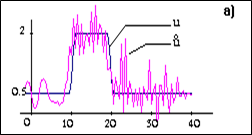
\includegraphics{{img/10/5.3.a}.png}
    \label{fig:5.3.a}
    \caption{без штучної в'язкості ($\alpha = 1$, $\beta=-1$, $\sigma=0.01$, $\sigma_1=0$, $\sigma_3=0$, $\sigma_2=0$; $h=0.5$, $\tau=0.25$)}
\end{figure}
\begin{figure}[H]
    \centering
    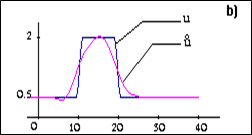
\includegraphics{{img/10/5.3.b}.png}
    \label{fig:5.3.b}
    \caption{із штучною в'язкістю ($\alpha = 1$, $\beta=-1$, $\sigma=0.01$, $\sigma_1=0.1$, $\sigma_3=0.1$, $\sigma_2=0$; $h=0.5$, $\tau=0.25$)}
\end{figure}
\begin{figure}[H]
    \centering
    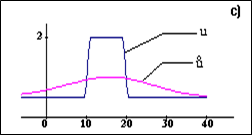
\includegraphics{{img/10/5.3.c}.png}
    \label{fig:5.3.c}
    \caption{із надто великою штучною в'язкістю ($\alpha = 1$, $\beta=-1$, $\sigma=0.01$, $\sigma_1=0.1$, $\sigma_3=0.1$, $\sigma_2=0$; $h=0.5$, $\tau=0.25$)}
\end{figure}

Тут і далі $u$ --- точний розв'язок, $\overset{\circ}{u}$ --- розв'язок, знайдений за допомогою ДС-методу (2.37), (2.38). На наступних малюнках представлені результати тестування ДС-алгоритмів із штучною в'язкістю ($a$ --- коефіцієнт при явній штучній в'язкості, $a_1$ --- коефіцієнт при неявній штучній в'язкості) на вказаних модельних задачах (схеми, в яких явні частини --- проти потоку, неявні частини --- за потоком).

\begin{minipage}[t]{.45\textwidth}
    \begin{figure}[H]
        \centering
        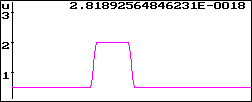
\includegraphics{{img/10/5.4}.png}
        \label{fig:5.4}
        \caption{\scriptsize $h=0.5$, $\tau=0.5$, $\sigma=2$, $a=0$, $a_1=0$}
    \end{figure}
\end{minipage}
\begin{minipage}[t]{.45\textwidth}
    \begin{figure}[H]
        \centering
        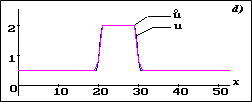
\includegraphics{{img/10/5.5}.png}
        \label{fig:5.5}
        \caption{\scriptsize $h=0.5$, $\tau=0.5$, $\sigma=0.01$, $a=0$, $a_1=0$}
    \end{figure}
\end{minipage}

\begin{minipage}[t]{.45\textwidth}
    \begin{figure}[H]
        \centering
        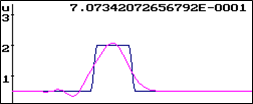
\includegraphics{{img/10/5.6}.png}
        \label{fig:5.6}
        \caption{\scriptsize $h=0.5$, $\tau=0.25$, $\sigma=1$, $a=1$, $a_1=1$}
    \end{figure}
\end{minipage}
\begin{minipage}[t]{.45\textwidth}
    \begin{figure}[H]
        \centering
        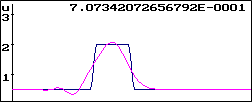
\includegraphics{{img/10/5.7}.png}
        \label{fig:5.7}
        \caption{\scriptsize $h=0.5$, $\tau=0.25$, $\sigma=0.01$, $a=0.1$, $a_1=0$}
    \end{figure}
\end{minipage}

\begin{minipage}[t]{.45\textwidth}
    \begin{figure}[H]
        \centering
        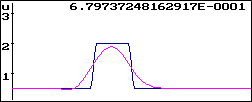
\includegraphics{{img/10/5.8}.png}
        \label{fig:5.8}
        \caption{\scriptsize $h=0.5$, $\tau=0.25$, $\sigma=0.01$, $a=0.1$, $a_1=0.1$}
    \end{figure}
\end{minipage}
\begin{minipage}[t]{.45\textwidth}
    \begin{figure}[H]
        \centering
        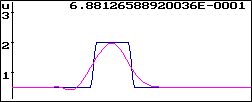
\includegraphics{{img/10/5.9}.png}
        \label{fig:5.9}
        \caption{\scriptsize $h=0.5$, $\tau=0.25$, $\sigma=0.01$, $a=0.1$, $a_1=0.05$}
    \end{figure}
\end{minipage}

\begin{minipage}[t]{.45\textwidth}
    \begin{figure}[H]
        \centering
        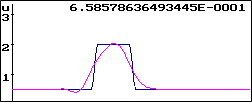
\includegraphics{{img/10/5.10}.png}
        \label{fig:5.10}
        \caption{\scriptsize $h=0.5$, $\tau=0.125$, $\sigma=0.01$, $a=0.5$, $a_1=0$}
    \end{figure}
\end{minipage}
\begin{minipage}[t]{.45\textwidth}
    \begin{figure}[H]
        \centering
        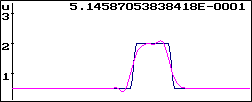
\includegraphics{{img/10/5.11}.png}
        \label{fig:5.11}
        \caption{\scriptsize $h=0.5$, $\tau=0.025$, $\sigma=0.01$, $a=2$, $a_1=2$}
    \end{figure}
\end{minipage}

\begin{minipage}[t]{.45\textwidth}
    \begin{figure}[H]
        \centering
        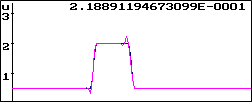
\includegraphics{{img/10/5.12}.png}
        \label{fig:5.12}
        \caption{\scriptsize $h=0.5$, $\tau=0.5$, $\sigma=100$, $a=1$, $a_1=0$}
    \end{figure}
\end{minipage}
\begin{minipage}[t]{.45\textwidth}
    \begin{figure}[H]
        \centering
        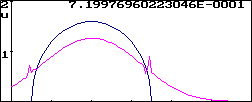
\includegraphics{{img/10/5.13}.png}
        \label{fig:5.13}
        \caption{\scriptsize $h=0.5$, $\tau=0.25$, $\sigma=1$, $a=1$, $a_1=1$}
    \end{figure}
\end{minipage}

\begin{minipage}[t]{.45\textwidth}
    \begin{figure}[H]
        \centering
        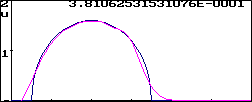
\includegraphics{{img/10/5.14}.png}
        \label{fig:5.14}
        \caption{\scriptsize $h=0.5$, $\tau=0.25$, $\sigma=0.01$, $a=0.1$, $a_1=0$}
    \end{figure}
\end{minipage}
\begin{minipage}[t]{.45\textwidth}
    \begin{figure}[H]
        \centering
        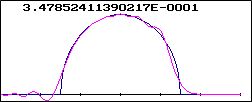
\includegraphics{{img/10/5.15}.png}
        \label{fig:5.15}
        \caption{\scriptsize $h=0.5$, $\tau=0.125$, $\sigma=0.01$, $a=0.1$, $a_1=0.05$}
    \end{figure}
\end{minipage}

\begin{minipage}[t]{.45\textwidth}
    \begin{figure}[H]
        \centering
        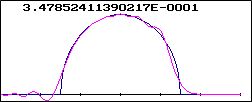
\includegraphics{{img/10/5.16}.png}
        \label{fig:5.16}
        \caption{\scriptsize $h=0.5$, $\tau=0.025$, $\sigma=0.01$, $a=0$, $a_1=0$}
    \end{figure}
\end{minipage}
\begin{minipage}[t]{.45\textwidth}
    \begin{figure}[H]
        \centering
        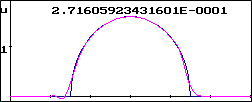
\includegraphics{{img/10/5.17}.png}
        \label{fig:5.17}
        \caption{\scriptsize $h=0.5$, $\tau=0.025$, $\sigma=0.01$, $a=2$, $a_1=2$}
    \end{figure}
\end{minipage}

\begin{minipage}[t]{.45\textwidth}
    \begin{figure}[H]
        \centering
        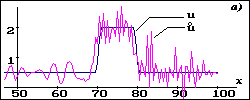
\includegraphics{{img/10/5.18}.png}
        \label{fig:5.18}
    \end{figure}
\end{minipage}
\begin{minipage}[t]{.45\textwidth}
    \begin{figure}[H]
        \centering
        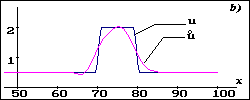
\includegraphics{{img/10/5.18.a}.png}
        \label{fig:5.18.a}
    \end{figure}
\end{minipage}

\begin{minipage}[t]{.45\textwidth}
    \begin{figure}[H]
        \centering
        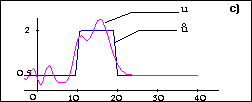
\includegraphics{{img/10/5.18.b}.png}
        \label{fig:5.18.b}
    \end{figure}
\end{minipage}
\begin{minipage}[t]{.45\textwidth}
    \begin{figure}[H]
        \centering
        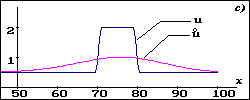
\includegraphics{{img/10/5.18.c}.png}
        \label{fig:5.18.c}
    \end{figure}
\end{minipage}

\begin{minipage}[t]{.3\textwidth}
    \begin{figure}[H]
        \centering
        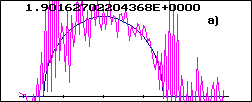
\includegraphics[width=\textwidth]{{img/10/5.19.a}.png}
        \label{fig:5.19.a}
    \end{figure}
\end{minipage}
\begin{minipage}[t]{.3\textwidth}
    \begin{figure}[H]
        \centering
        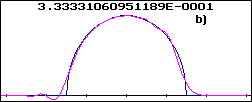
\includegraphics[width=\textwidth]{{img/10/5.19.b}.png}
        \label{fig:5.19.b}
    \end{figure}
\end{minipage}
\begin{minipage}[t]{.3\textwidth}
    \begin{figure}[H]
        \centering
        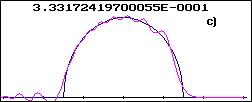
\includegraphics[width=\textwidth]{{img/10/5.19.c}.png}
        \label{fig:5.19.c}
    \end{figure}
\end{minipage}

\section{Завдання для самостійної роботи}

\shortHomeworkDescription{Дослідити перше диференціальне наближення телеграфного рівняння. Встановити наявність схемної в'язкості.}

\end{document}
